\chapter{Virtualization - Hypervisor (Virtual Machine Monitor - VMM)}
\label{chap:Hypervisor}

%\section{Virtualization - Hypervisor (Virtual Machine Monitor - VMM)}

Hypervisor is the agent that helps you create virtual machines.
Hypervisor is the guy who creates and runs the guest machine and provide the
host’s resource to the guest. 

\section{Review}

\subsection{User-mode Linux (UML)}

UML allows a Linux kernel to run as a user process (like any other Linux
process, such as Emacs or Vim) within a "host" Linux operating system.

This interesting technology has a number of advantages, such as the ability to
run any recent UML-enabled kernel of choice (including one different from the
kernel of the host system) and the ability to debug the kernel of the guest
system more easily.



\subsection{Full virtualization}

When many people think of virtualization, they think about full virtualization
software that emulates a virtual machine all the way down to the hardware level
and lets an operating system run on top of that emulated hardware. This is the
approach taken by several well-known software packages such as VMware, QEMU, and
Bochs.

Example of hypervisors
\begin{enumerate}
  \item QEMU 
  
  \item KVM 
  
  KVM helps QEMU to access hardware virtualization features on different
  architectures.
  It also adds the acceleration feature to the QEMU process. So, in short, when
  they are together, QEMU is the hypervisor/emulator and KVM is the accelerating
  agent.
  
\end{enumerate}

Full virtualization software does extensive virtualization of hardware,
including the processor, BIOS, and I/O devices. One of the advantages of this
approach is that just about any operating system can be run on the virtual
hardware. One disadvantage is that emulating down to the hardware layer involves
a lot of overhead, which usually results in a noticeable performance degradation
for the guest and host operating system.

\subsection{paravirtualization}

Virtualization technologies such as KVM and Xen, which started by booting
separate virtual systems on emulated hardware and then attempted to lower their
overhead via paravirtualization and related mechanisms.


Recent years have seen a lot of interest in another virtualization technique
called paravirtualization. With paravirtualization, virtual machines run inside
a virtual machine monitor (VMM), or hypervisor, and access its services through
a software interface.

Paravirtualization is actually an old technique dating back to IBM mainframes,
but lately it's increasingly being applied to personal computers with software
such as Parallels Workstation and Xen.


Paravirtualization does have drawbacks, though, as it typically requires either
the guest operating system to be modified to support the hypervisor, or specific
hardware support in newer Intel and AMD processors.


\section{Virtualization \& Hypervisors}

You are running on Windows platform, but you want to test software running on
Linux platform on the same machine, without rebooting the PC; then it comes
{\bf virtualization} and the tools are called {\bf hypervisor}.

\subsection{Virtualization}


{\bf Virtualization} refers to the creation of a virtual (rather than actual)
version of something, e.g. an O/S or a machine or a storage device or a network
resource.
\begin{itemize}
  \item \textcolor{red}{O/S virtualization} (or virtual machine): the most
  prevalent form of virtualization

  \item \textcolor{red}{Application Virtualization} (aka thin clients): you run
  a program locally, but all the binaries, running states, \ldots are stored on,
  managed, and delivered by a remote machine. Your local machine provide the CPU
  and RAM required to run the application, but nothing is installed locally on
  your own machine.
  
  
  \item \textcolor{red}{Application Server Virtualization} (often used in
  advanced load balancing): one server is presented to the outer-world, hiding the
  availability of multiple servers. This public server runs as a reverse 
  proxy load balancer (an appliance or servie that provide access to many
  different application services transparently) and provides a virtual interface
  (Virtual IP or VIP), represent itself as the actual web server.
  
% multiple web servers or applications are managed by a load balancer
   \item \textcolor{red}{Management virtualization} : (1) virtual IP management
   and segmentation, e.g. VLAN (a single Ethernet port may support multiple
   virtual connections from multiple IP addresses and networks, but they are
   virtually segmented using VLAN tags, e.g. eth0:1 virtual network adapters).
   (2) virtual routing tables (typically a routing table and an IP network share
   a 1:1 relationship, even though a single port may host multiple virtual
   interfaces).
   
   Each virtual IP connection over this single physical port is independent and
   unaware of other's existence, but the switch is aware of each unique
   connection and manage each one independently.
   
   
   
   
   \item \textcolor{red}{Network virtualization}: 
   
 %  \item 
\end{itemize}
\url{https://www.f5.com/pdf/white-papers/virtualization-defined-wp.pdf}

\subsection{Hypervisor}
\label{sec:hypervisor}


A {\bf hypervisor} is a class of software  which is tasked with creating,
releasing, and managing the resources of "guest" operating systems, or virtual
machines. Hypervisor is used on VPS (Sect.\ref{sec:VPS}). Examples of
hypervisors are VMware (Sect.\ref{sec:VMWare_ESXi}), HyperV
(Sect.\ref{sec:Hyper-V}).

{\bf Hypervisor} is a system comprised of computer software, firmware + hardware
that creates a virtual machine that enable deploying any guest operating system
easily, Fig.\ref{fig:Hypervisor}. 

\section{Type-1 and Type-2 hypervisors}
\label{sec:hypervisor-type-I}
\label{sec:hypervisor-type-II}


There are two types of hypervisor (Sect.\ref{sec:hypervisor}): Type-1 and Type-2.


As Type-1 is faster, Type 1 hypervisors provide {\it server} (i.e. no GUI)
virtualization on bare metal hardware, whereas Type 2 hypervisors typically
provide {\it desktop} virtualization based on an existing operating system.



\begin{itemize}
  
  \item {\bf Type-1} (bare-metal hypervisor): the hypervisor runs directly on
  the host's hardware to control the hardware and manage the guest O/S. For this
  reason, they are aka {\bf bare metal hypervisors}. The guest O/S runs as a
  process on the host.
  
\begin{verbatim}
your apps
----------------
Guest O/S
----------------
Type-I hypervisor
----------------
hardware
\end{verbatim}
  

  Example: Oracle VM Server for SPARC, Oracle VM Server for x86, Microsoft
  Hyper-V 2008/2012 (Sect.\ref{sec:Hyper-V}).
  
  Xen hypervisor project is the only open-source Type-1 hypervisor (Sect.\ref{sec:Xen}).
  
  \item {\bf Type-2} (hosted hypervisor): these hypervisors run like a
  conventional computer programs, and provides the environment to host a guest
  O/S.  

\begin{verbatim}
your apps
----------------
Guest O/S  [e.g. Linux]
----------------
Type-2 hypervisor  (provide software emulation, mapping from Linux-based to Windows-based)
----------------
host O/S [e.g. Windows]
----------------
hardware
\end{verbatim}

Early virtualization efforts relied on software emulation to replace hardware
functionality. But software emulation can be a slow and inefficient process.
Because many virtualization tasks were handled through software, VM behavior and
resource control were often poor, resulting in unacceptable VM performance on
the server. Sect.\ref{sec:virtualization_hardware} discusses how ntel Corp. and
AMD addressed this problem by creating processor extensions that could offload
the repetitive and inefficient work from the software.


  
  Example: VirtualBox, VMWare Workstations programs.
\end{itemize}

The computer on which hypervisor is running is called the {\bf host machine}.
The hardware/firmware/software - collective form a virtual machine - on which
the guest O/S running is not necessary the same as the
hardware/firmware/software of the host machine, as the hyeprvisor can emulate
that. Each virtual machine is called a {\bf guest machine}. Multiple instances
of a variety of O/S may share the virtualized hardware resources.
\url{http://www.ibm.com/developerworks/cloud/library/cl-hypervisorcompare/}
 
\begin{figure}[hbt]
  \centerline{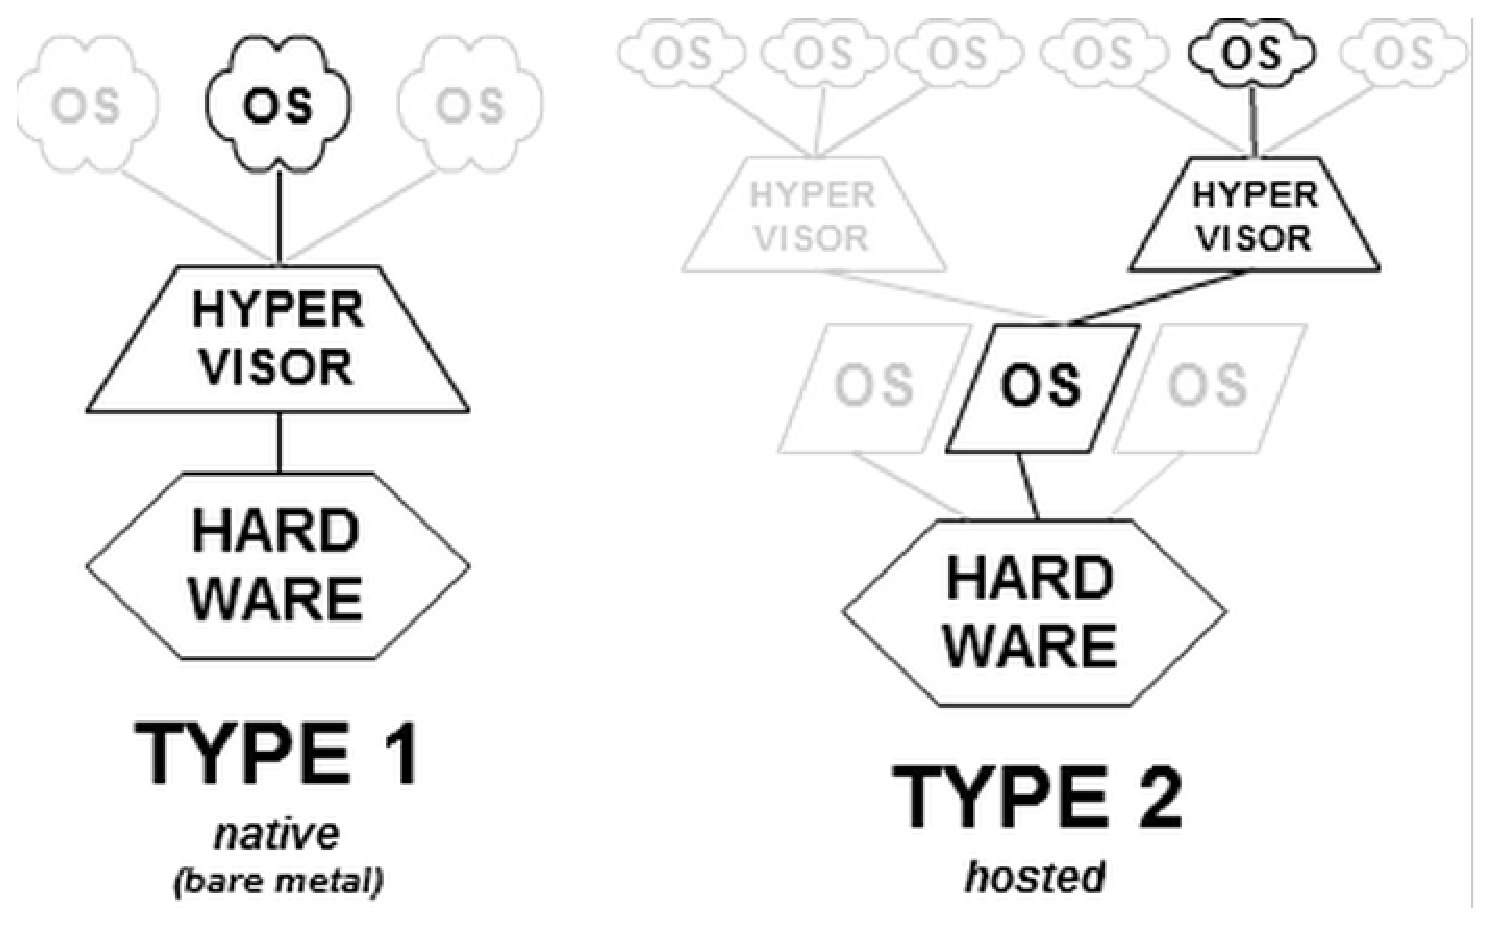
\includegraphics[height=6cm,
    angle=0]{./images/Hypervisor.eps}}
\caption{Type-1 and Type-2 hypervisors}
\label{fig:Hypervisor}
\end{figure}

All hypervisors are not made equal, but they all offer similar features.
Understanding the features they have as well as the guest operating systems each
supports is an essential aspect of any hardware virtualization hypervisor
selection process.

 Review:
\url{http://www.flexiant.com/2014/02/12/hypervisor-comparison-kvm-xen-vmware-hyper-v/}

\section{Hardware support for virtualization}
\label{sec:virtualization_hardware}


Early virtualization efforts relied on software emulation to replace hardware
functionality which is slow. Both Intel Corp. and AMD addressed this problem by
creating processor extensions that could offload the repetitive and inefficient
work from the software. By handling these tasks through processor extensions,
traps and emulation of virtualization, tasks through the operating system were
essentially eliminated, vastly improving VM performance on the physical server.


To enable sharing hardware easily, extra hardware components were granually
added to manage that, e.g. since 2006 Intel (VT-x, codename Vanderpool) and
since 2004 for AMD (AMD-V, codename Pacifica) to allow simpler virtualization
software. Later on, many other technologies have been developed.

\begin{itemize}
  
  \item {\bf first generation}: AMD-V and Intel VT-x
  
  \item {\bf second generation}: AMD-V/RVI (Rapid Virtualization Indexing, or
  former name Nested Page Tables) which is adopted by Intel under a different name:
  Extended Page Tables (VT-x/EPT).
  
NOTE: A study by VMware found that RVI offers up to 42\% gains in performance
compared with software-only (shadow page table), and one by RedHat found 200\%
in performance for OLTP benchmark.
   
\end{itemize}

To check on Ubuntu
\begin{verbatim}
egrep -c '(vmx|svm)' /proc/cpuinfo
\end{verbatim}
\verb!0! = no hardware virtualization. If 1, it supports, but make sure it is
enabled in the BIOS. 

\subsection{AMD-V and Intel VT-x}
\label{sec:AMD-V}

\begin{enumerate}
  \item in 2004: AMD-V (AMD virtualization) is a set of hardware extensions for the X86 processor architecture.

added to AMD's Pacifica 64-bit x86 processor designs
  
in 2006: 2006, AMD's Athlon 64 X2 and Athlon 64 FX processors appeared with
AMD-V technology, and today, the technology is available on Turion 64 X2,
second- and third-generation Opteron, Phenom and Phenom II processors.
  
\end{enumerate}




Open BIOS, you can enable the feature:	Intel Virtualization Technology (also
known as Intel VT) or AMD-V on your CPU chip. 

When enabled and the CPU chip supports, an input/output memory management unit
(IOMMU) allows guest virtual machines to directly use peripheral devices, such
as Ethernet, accelerated graphics cards, and hard-drive controllers, through DMA
and interrupt remapping. This makes the guest O/S runs much faster, than
tradititional virtual machines.


\subsection{AMD-V/RVI and Intel VT-x/EPT}
\label{sec:AMD-V/RVI}

\url{https://support.amd.com/en-us/kb-articles/Pages/GPU120AMDRVICPUsHyperVWin8.aspx}

AMD processors that support AMD Virtualization (AMD-V) Technology with Rapid
Virtualization Indexing (RVI), also known as nested page tables or Second Level
Address Translation (SLAT) necessary to support Hyper-V virtualization
technology in Microsoft Windows 8.



\section{KVM (type-1)}
\label{sec:KVM}

{\bf KVM} (Kernel-based Virtual Machine) is the Linux-based Open-source
Hypervisor, first introduced in 2007. KVM supports native virtualization on
processors with hardware virtualization extensions (e.g. x86 processors, ARM,
IA-64, x86-64, PowerPC, S/390), and guest operating systems including many
variations of Linux, BSD, Solaris, Windows, Haiku, ReactOS, and the AROS
Research Operating System (there's even a modified version of qemu that can use
KVM to run Mac OS X).

It is being used in Redhat Enterprise Virtualization (RHEV).
\url{http://www.linux-kvm.org/page/Main_Page}

To run KVM, you need a processor that supports hardware virtualization
(Sect.\ref{sec:virtualization_hardware}). To setup KVM in Ubuntu
\url{https://help.ubuntu.com/community/KVM/Installation}

\section{Xen (Type-1)}
\label{sec:Xen}
\label{sec:Xen-hypervisor}


An open source hypervisor which originated in a 2003 Cambridge University
research project. Its \verb!dom0! host runs on Linux, which in turns run on Xen.
It was originally supported by XenSource Inc, which was acquired by Citrix Inc in 2007.

\ref{sec:hypervisor-type-I}

\section{VMWare's ESXi (type-1, for server)}
\label{sec:VMWare_ESXi}

VMware ESX's enterprise software hypervisors (VMWare vSphere) run directly on
server hardware without requiring an additional underlying operating system.
VMware's hypervisor is very mature and extremely stable.

The obsolete version (since 2011) is VMWare Server.

\section{VMWare Player (for desktop)}
\label{sec:VMWare_Player}

VMWare Player:
\url{https://my.vmware.com/web/vmware/free#desktop_end_user_computing/vmware_player/4_0}

If you run Linux as the guest O/S, it may ask you to install
Linux tool.

To enable shared-folder, we use
\url{https://www.vmware.com/support/ws5/doc/ws_running_shared_folders.html}

VMWare Player
\begin{itemize}
  \item 6.0: support new O/S (Windows 8.1), VM (16 vCPUs, 8TB, virtual SATA controller, USB3)
\end{itemize}

\section{Hyper-V}
\label{sec:Hyper-V}

Hyper-V is a commercial hypervisor provided by Microsoft, running on Windows but
can host any O/S supported by the hardware platform. 


\section{App-V (app virtualization)}
\label{sec:App-V}

Microsoft Application Virtualization (App-V, Softricity SoftGrid) is an 
application virtualization and application streaming solution from Microsoft.

App-V technology allows applications to be deployed ("streamed") in real-time to
any client from a virtual application server, i.e. no need to install locally
(although a standalone deployment is still supported).

The App-V client needs to be installed on the client machines and application
data that is stored on the virtual application server is installed (streamed) to
the client cache on demand when it is first used, or pre-installed in a local
cache.

Different versions of the same application can be run under App-V concurrently
and so that mutually exclusive applications can co-exist on the same system.

\url{https://en.wikipedia.org/wiki/Microsoft_App-V}

\section{z/VM (IBM, type-1)}

z/VM runs on IBM's zSeries and can be used to support large numbers (thousands)
of Linux virtual machines.

\section{PowerVM (type-2)}

PowerVM is a feature of IBM POWER5, POWER6, and POWER7 servers, support
provided for it on IBM i, AIX, and Linux O/S.

\section{VirtualBox (type-2)}
\label{sec:VirtualBox}

 VirtualBox works on multiple platforms with easy installation and setup.  It
 can run on Windows, Linux, Macintosh, and Solaris hosts, and supports host
 installation of Windows (NT 4.0, 2000, XP, Server 2003, Vista, Windows 7,
 Windows 8), DOS/Windows 3.x, Linux (2.4, 2.6 and 3.x), Solaris and OpenSolaris,
 OS/2, and OpenBSD.
 
Among the compelling features, VirtualBox makes running multiple OS guests easy;
your limits are primarly dictated by your system memory and CPU capability.

\chapter{Isolation (O/S-level virtualization) - Container}

\section{History of container runtime}
\label{sec:container-technology-history}

Since system administration is a difficult task, many tools have been developed
to make life easier for the administrator. These tools often enhance the way
systems are installed, configured, and maintained. One of the tools which can be
used to enhance the security of a FreeBSD system is jails (Sect.\ref{sec:jail}).

This {\bf Operating-system-level virtualization},
also known as containerization, refers to an operating system feature in which
the kernel allows the existence of multiple isolated user-space instances.

So, a {\bf container} is like a virtual environment, in that a software can
run in isolation of other software running on the physical host machine.
There is no spec specifying what a container should implement.
There are several Linux-based Containers projects:

The container technology is not new, but is getting so popular recently
primarily because kernel support is now available in Linux (namespace and
cgroups) kernel 3.8 (Feb 2013).

There have been different implementations of a container runtime to support
launching a container

\begin{enumerate}
  
  \item chroot - Sect.\ref{sec:chroot}
  
  \item Jails (FreeBSD) - Sect.\ref{sec:jail}
  \item Zones (Solaris) - Sect.\ref{sec:zones-Solaris}
  
  \item Google container: use cgroup of the kernel (Sect.\ref{sec:cgroups})
  
  \url{https://github.com/google/lmctfy}

  \item OpenVZ (depends on custom kernel) - Sect.\ref{sec:OpenVZ}
  \item WPARs (AIX O/S - Workload PARtitions)
  
  \item Linux VServer (depends on custom kernel)
  
  \url{http://linux-vserver.org/}
  
  
  \item OpenVZ: based on modified kernel - Sect.\ref{sec:OpenVZ}
  
  
  \item Linux-based container (LXC): Sect.\ref{sec:LXC} from 2014
  
  \item Docker - Sect.\ref{sec:Docker} - the company and the technology it provides that really makes
  container-like technology becomes popular.
\end{enumerate}

Review: \url{http://ramirose.wix.com/ramirosen} 


\subsection{Linux namespace}

In namespaces, you start with no isolation, from zero, and you add whatever you
want — mount, PID, network, hostname, user, IPC namespaces.


In Linux namespaces,  user isolation is done with weird UID mapping ("uid
1 in the container is uid 1000001 outside") and PID isolation I don't even know
how, jails are at their core just one more column in the process table. PID,
UID, and now JID (Jail ID). (The host is JID 0.) No need for weird mappings, the
system just takes JID into account when answering system calls.



Jails are actually very similar to Linux namespaces / unshare. But unlike Linux
namespace (which starts with nothing), in jails, you start with a reasonable
secure baseline — processes, users, POSIX IPC and mounts are always isolated.
But! You can isolate the filesystem root — or not (by specifying /). You can
keep the host networking or restrict IP addresses or create a virtual interface.
You can isolate SysV IPC (yay postgres!) — or keep the host IPC namespace, or
ban IPC outright. See? The interesting parts are still flexible! Okay, not as
flexible as "sharing PIDs with one jail and IPC with another", but still.

\url{https://news.ycombinator.com/item?id=13982620}


\subsection{1979: Unix V7 with chroot}
\label{sec:chroot}

During the unix history of containers development of Unix V7 in 1979, the chroot
system call was introduced, changing the root directory of a process and its
children to a new location in the filesystem. This advance was the beginning
process isolation: segregating file access for each process.


\verb!chroot! utility is used to change the {\it root directory} (which is '/'
by default) of a running process and all of its children, to some subtree of the larger file system.

Example: change the root to /mnt/arch and we have defined the shell.
\begin{verbatim}
chroot /mnt/arch /usr/bin/bash
\end{verbatim}

\verb!chroot! modifies pathname lookups for a process and its children so that
any reference to a path starting '/' will effectively have the new root, which
is passed as the single argument, prepended onto the path.


This technique is commonly used to improve computer security by placing a
vulnerable server process in a chroot jail that is isolated from the rest of the
system.

NOTE: Calls to chroot() do not stack, with additional calls essentially
overwriting the existing one.


A process/command that runs in such a modified environment cannot access files
outside the given root directory. If we change from '/' to \verb!/chroot/named! as
root directory, then within this chroot jail, /etc/passwd, for example, would
map to /chroot/named/etc/passwd in the main file system.

SYNTAX:
\begin{verbatim}

chroot /path/to/new/root /path/to/server

chroot [options] /path/to/new/root /path/to/server

	–userspec=USER:GROUP : This option describe the user and group which is to be used.
	
	–groups=G_LIST : It describe the supplementary groups as g1,g2,..,gN.
\end{verbatim}

Example:
\begin{verbatim}
# create a “jail” directory inside the “home” directory, which will be our new root.

mkdir $HOME/jail


mkdir -p $HOME/jail/{bin, lib64}
cd $HOME/jail

# copy essential files, 
# /bin/bash and /bin/ls into $HOME/jail/bin/ location

cp -v /bin/{bash, ls} $HOME/jail/bin


# find what other essential libraries
ldd /bin/bash

# ... and copies these libraries
cp -v libraries/displayed/by/above/command $HOME/jail/lib64

# finally, issue 'chroot'

sudo chroot $HOME/jail /bin/bash
\end{verbatim}


%Suppose you're running a process, from the directory 'A', now, from within the
%process, you want the process to receive directory 'B' as the base-folder, then
%you issue 'chroot' command within the process.

Processes created in the chrooted environment can not access files or resources
outside of it.  In a traditional chroot environment, processes are only limited
in the part of the file system they can access. The rest of the system
resources, system users, running processes, and the networking subsystem are
shared by the chrooted processes and the processes of the host system.


\begin{mdframed}


The use of the term "chroot jail" in the manpage is unfortunate as it may help
perpetuate a common misconception about chroot(). It often gets mentioned in the
same context as the "jail" calls for the BSDs, but it has little in common with
them.

\url{https://lwn.net/Articles/252794/}

Chroot was added to BSD in 1982. 
\url{https://www.freebsd.org/cgi/man.cgi?query=chroot&sektion=2&manpath=freebsd-release-ports}
\end{mdframed}

\subsection{2000: jail utility - FreeBSD Jail}
\label{sec:jail}

jail have been available since FreeBSD 4.X, and is buit upon the \verb!chroot!
concept (Sect.\ref{sec:chroot}) which has long been supported by many UNIX
kernels, including the Linux kernel.

COMMAND SYNTAX:
\url{https://www.freebsd.org/cgi/man.cgi?query=jail&sektion=8&manpath=freebsd-release-ports}

\verb!jail! helps to create a containerized environment for a running process
and its children like \verb!chroot!; but with more complexity.
A BSD jail is a mini-virtualization that partitions a system into multiple
virtual systems each of which can have its own root account. chroot() has none
of that sophistication.

\verb!chroot! is suited to easy tasks which do not require much flexibility or
complex, advanced features. With chroot, it only isolate the file systems, while
the rest of the system resources, system users, running processes, and the
networking subsystem are shared by the chrooted processes and the processes of
the host system.

Jails expand this model by virtualizing access to the file system, the set of
users, and the networking subsystem. More fine-grained controls are available
for tuning the access of a jailed environment. Jails can be considered as a type
of operating system-level virtualization.

In each containerized environment or virtual system, jail provides it with an
own set of users and their own root account which are limited to the jail
environment. The root account of a jail is not allowed to perform operations to
the system outside of the associated jail environment.
\url{https://linux.die.net/man/8/jailkit}

IN SUMMARY: A jail is characterized by 4 elements
\begin{enumerate}
  \item a new root directory (like chroot provides)
  
  A directory subtree: the starting point from which a jail is entered. Once
  inside the jail, a process is not permitted to escape outside of this subtree.
  
  \item a hostname: which will be used by the jail.
  
  \item an IP address: which is assigned to the jail. The IP address of a jail
  is often an alias address for an existing network interface.

  \item a  command: the path name of an executable to run inside the jail. The
  path is relative to the root directory of the jail environment.
  
\end{enumerate}

Also, jails have their own set of users and their own root account which are
limited to the jail environment. The root account of a jail is not allowed to
perform operations to the system outside of the associated jail environment.

\url{https://www.freebsd.org/doc/handbook/jails.html}

% Jailkit is a set of utilities that can limit user accounts to a specific
% directory tree and to specific commands
% \begin{itemize}
%    \item Jailkit is a set of utilities to limit user accounts to specific files using chroot() and or specific commands.
%  
%   \item  A jail is a directory tree that you create within your file system; the
%   user cannot see any directories or files that are outside the jail directory
% \end{itemize}
% \urk{https://olivier.sessink.nl/jailkit/index.html#intro}

Example: 
\verb!jk_cp! can be used to copy a file or device into a jail.
\begin{verbatim}

mkdir /home/sftproot
chown root:root /home/sftproot

chmod 0755 /home/sftproot

# quickly create a jail with several files or directories needed for a specific
# task or profile.

jk_init -j /home/sftproot jk_lsh
jk_init -j /home/sftproot sftp
jk_init -j /home/sftproot scp

# Create the account
jk_addjailuser -j /home/sftproot test

# Edit the jk_lsh configfile in the jail; see man jk_lsh.

# You can use every editor you want; I choose 'joe'
joe /home/sftproot/etc/jailkit/jk_lsh.ini

# Restart jk_socketd so that log messages are transferred
killall jk_socketd
jk_socketd

# Test the account
sftp test@localhost
# Check the logs to see if everything is correct
tail /var/log/daemon.log /var/log/auth.log

\end{verbatim}



The jail utility creates new jails, or modifies or	removes	existing
jails.   \url{https://www.freebsd.org/doc/handbook/jails.html}

A jail (or	``prison'') is specified via parameters	on the command
line, or in the jail.conf file.
     

FreeBSD Jails allows administrators to partition a FreeBSD computer system into
several independent, smaller systems – called “jails” – with the ability to
assign an IP address for each system and configuration.

This achieve clear-cut separation between its services and those of its
customers for security and ease of administration.

\subsection{2001: util-vserver utility - Linux VServer (similar to FreeBSD Jail)}

Linux-VServer allows you to create lightweight virtual machines with little
overhead and great performance, while still providing increased security and
fault isolation. You can use it to create a secure and fault-tolerant system
without investing in additional hardware.
 
\verb!jail! was developed for Free BSD O/S. In GNU/Linux systems, an equivalent
system called Linux-VServer was developed to provide virtualization for
GNU/Linux systems, i.e. a simple way to run several virtual servers on one piece
of physical hardware.

Linux VServer allows to run multiple virtual units at once. Those units are
sufficiently isolated to guarantee the required security, but utilize available
resources efficiently, as they run on the same kernel.
\url{http://www.linux-vserver.org/Welcome_to_Linux-VServer.org}

Linux-VServer is composed of two parts: Code in the kernel (i.e. require
patching the Linux kernel) to support security contexts, and userspace tools for
creating and managing virtual servers. Experimental patches are still available,
but the last stable patch was released in 2006. Linux-VServer, and similar
software like OpenVZ, take a "lightweight" approach to virtualization,
essentially segmenting a single Linux kernel environment into virtual machines
with separate file systems, process tables, and network addresses.

As a result, the virtual machines, often called security contexts or Virtual
Private Servers (VPS) in Linux-VServer parlance, can run at nearly the full
speed of the underlying physical hardware.
Unlike some other virtualization approaches, all the virtual servers run under
the control of the same kernel. This minor limitation is often outweighed by the
increase in performance that you can achieve by running a single kernel

Also keep in mind that although you're limited to a single kernel for all your
virtual machines, there is no problem with running different Linux distributions
in your virtual machines (as long as those Linux distributions can work with the
chosen kernel).


A Linux kernel on the host O/S needs to have support for VServer security
contexts. You can either download a kernel built with this support, or you can
download a VServer patch that you can apply to your kernel source code before
building.
\url{https://www.linux.com/news/installing-linux-vserver}
 
 
\subsection{2004: zones -  Solaris Zones (formerly Solaris Containers)}
\label{sec:zones-Solaris}

Solaris Containers (including Solaris Zones) is an implementation of operating
system-level virtualization technology for x86 and SPARC systems, first released in 2005.

Oracle Solaris Zones technology is an Oracle Solaris feature that first showed
up in Solaris Express and Oracle Solaris 10 3/05 and was called Oracle Solaris
Containers. With Oracle Solaris 11, we now officially call the technology Oracle
Solaris Zones.


Oracle Solaris Zones and Linux Containers are virtualization technologies at the
application level, so they are "above" the OS kernel. With Oracle Solaris Zones
and Linux Containers, there is one OS kernel that is shared by many zones or
containers.

\url{https://www.oracle.com/technical-resources/articles/it-infrastructure/admin-zones-containers-virtualization.html}

Solaris Zones are more designed and an evolution from FreeBSD Jails.
We could say a zone is a "sandbox" that provides a playground for an
application.
\begin{enumerate}
  
  \item The global zone holds the Oracle Solaris kernel, the device drivers and
  devices, the memory management system, the file system and, in many cases, the
  network stack.
  
  The global zone sees all physical resources and provides common access to
  these resources to the non-global zones.
  Looking from the global zone, a non-global zone is just a bunch of processes
  grouped together by a tag called a zone ID.
  
  
  \item The other zones are called non-global zones and are isolated from each
  other, but they all share one global zone. Non-global zones have their own
  file systems, process namespace, security boundaries, and network addresses.
  
  The non-global zones appear to applications like separate Oracle Solaris
  installations.
  
   Based on requirements, non-global zones can also have their own network stack
   with separate network properties. And, yes, there also is a separate
   administrative login (root) for every non-global zone, but even as a
   privileged user, there is no way to break into one non-global zone from a
   neighboring non-global zone. 
  
\end{enumerate}

Solaris Zones are included in the Solaris 11 Common Criteria Evaluation for the
virtualisation extension (VIRT) to the OSPP. Solaris Zones are also the
foundation of our multi-level Trusted Extensions feature and is used for
separation of classified data by many government/military deployments around the
world. \url{https://blogs.oracle.com/solaris/overview-of-solaris-zones-security-models-v2}


The first public beta of Solaris Containers was released that combines system
resource controls and boundary separation provided by zones, which were able to
leverage features like snapshots and cloning from ZFS.

%\subsection{Solaris Zones (2005+)}

A zone is a virtualized operating system environment created within a single
instance of the Solaris OS. Within a zone, the operating system is represented
to the applications as virtual operating system environments that are isolated
and secure. The applications run in different zones with complete isolation,
while the underlying operating system resources are centrally managed and
administered.


%\subsection{2005: Open VZ}
\subsection{2005: OpenVZ (partial type-2: container hypervisor)}
\label{sec:OpenVZ}

OpenVZ (Open Virtuzzo) is an operating system-level virtualization technology
for Linux which uses a patched Linux kernel for virtualization, isolation,
resource management and checkpointing. The code was not released as part of the
official Linux kernel.


It is possible to run production containers today, but not with
the mainline kernel. Instead, one can use the modified kernel provided by the
open source OpenVZ project.  
\url{http://lwn.net/Articles/524952/}


The \verb!libvirt! library makes it possible to start up an application in a
container.

It has a modified Linux kernel (meaning host systems can only be some flavor of
GNU/Linux) that is tailored to support OpenVZ containers.

The system containers are containers which offer an environment as close to
possible as the one you'd get from a VM but without the overhead that comes with
running a separate kernel and simulating all the hardware (see
Sect.\ref{sec:linuxcontainers.org}).

\subsection{2006: cgroups - Linux feature (formerly Process Containers)}
%\label{sec:cgroups}

Check the Sect.\ref{sec:cgroups} in Sys-admin book.


\subsection{2008 (released 2013): liblxc library - Linux Containers - LXC (partial type-2)}
\label{sec:LXC}

Based on the new features of Linux kernels,  the Linux Containers project
started around 2006 to provide light-weight virtualization to the Linux kernel
as an external set of patches to the Linux kernel. It was first implemented in
2008 using
\begin{enumerate}
  \item cgroups - Sect.\ref{sec:cgroups}
  
   Linux kernel's control groups ("Cgroups") subsystem is used by LXC 
   to provide resource management
    
  
  \item Linux namespaces (Sect.\ref{sec:namespaces}),
  
  LXC provides resource isolation through process namespaces. 
  
\end{enumerate}
It works on a single Linux kernel without requiring any patches.

Linux Containers offer essentially native performance, and you can efficiently
manage resource allocation in real time.

\textcolor{red}{IMPORTANT}: Unlike full virtualization solutions and similar to
Oracle Solaris Zones, LXC will not let you run any other non-Linux operating
systems (such as proprietary operating systems or other types of UNIX). However,
you are able to run different Linux distributions on the same host kernel in
different containers. For example, you could run an instance of Oracle Linux 5
inside a container hosted on an Oracle Linux 6 system running the Unbreakable
Enterprise Kernel release 2.
\url{https://www.oracle.com/technical-resources/articles/it-infrastructure/admin-zones-containers-virtualization.html}

Unprivileged containers are containers that are run without any privilege. This
requires support for user namespaces in the kernel that the container is run on.
LXC was the first runtime to support unprivileged containers after user
namespaces were merged into the mainline kernel.
\begin{verbatim}
apt-get install lxc libvirt0 libpam-cgroup libpam-cgfs bridge-utils

\end{verbatim}

LXC was delivered in \verb!liblxc! library and provided language bindings for
the API in Python3, Python2, Lua, Go, Ruby, and Haskell. \verb!liblxc! library -
LXC (LinuX Containers) was the first, most complete implementation of a runtime
environment for a Linux container manager.
LXC is used as the default runtime for LXD, a container hypervisor exposing a
well-designed and stable REST-api on top of it (Sect.\ref{sec:LXD}).


Like OpenVZ (Sect.\ref{sec:OpenVZ}), LXC is a container technology.
LinuX Containers (LXC) is an operating system-level virtualization method for
running multiple isolated Linux systems (containers) on a single control host
(LXC host).

LXC's main focus is system containers. That is, containers which offer an
environment as close as possible as the one you'd get from a VM but without the
overhead that comes with running a separate kernel and simulating all the
hardware. This is achieved through a combination of kernel security features
such as namespaces, mandatory access control and control groups.



There is no need for a separate kernel under LXC since it takes root
in the host kernel. Like OpenVZ, LXC uses the resource management and
checkpointing of the host kernel. 

\begin{itemize}
 
  \item LXC 3.0: 
  
  \item LXC 2.0
   
  \item LXC 1.0 was released in February (20.2.2014).
  
  
LXC is included in Ubuntu 14.04.

  \item  LXC-0.9.0 was released, in April 2013.
  
 \end{itemize}

LXC helps to build a light-weight Linux virtual machines (i.e. an O/S container)
that you can launch this virtual machine on any computing machine; while Dockers
helps to build a container for an application (application container) so that it
contains required packages (with the minimal O/S components) so that the
application can run the same everywhere (Sect.\ref{sec:Docker}).

The LXC Project is supported by Ubuntu and powers Ubuntu Juju
(Sect.\ref{sec:Juju}). LXC is actively developed but not well documented beyond
Ubuntu. \url{http://www.flockport.com/lxc-vs-docker/}

The LXC project provides base OS container templates and a comprehensive set of tools for
container lifecycle management. It is currently led by a 2 member team, Stephane
Graber and Serge Hallyn from Ubuntu.   

LXC consists of a variety of container templates, standard tools for managing
containers, bindings for multiple languages (Ruby, Python, Go, Lua, etc), and
the \verb!liblxc! library (\verb!libvirt! is considered an alternative library).
LXC is free software, most of the code is released under the terms of the GNU
LGPL license

Docker (Sect.\ref{sec:Docker}) as developped by Docker, Inc is a container
system based on LXC container technology, has exploded in popularity.
\url{http://www.zdnet.com/article/ubuntu-is-working-on-a-new-secure-container-hypervisor-lxd/}

\subsection{-- install in Debian-based O/S}


\subsection{-- networking}

NOTE: most container templates configure the first interface to use DHCP by default.

\textcolor{red}{LXC 2.0+}:
Stretch ships with a new major release of LXC which also includes a helper for
easier networking setup called lxc-net lxc-net allows you to set up a simple
bridge for your containers, providing a DHCP-and-NATed IPv4 network. IPv6
support currently (in Stretch) requires manual configuration.

\url{https://wiki.debian.org/LXC}
 
\textcolor{red}{LXC 1.0+}:
 
Debian's packages do not ship any default network setup for containers
(/etc/lxc/default.conf contains lxc.network.type = empty).
If you want to have network in your containers (and you usually do), you will
have to either change the global default or configure each individual container.
You will also probably will have to setup a bridge, firewall and maybe DHCP (see
below for details how to do this).




\subsection{-- LinuxContainers.org: LXC, LXD, LXCFS, CGManager}
\label{sec:linuxcontainers.org}

Linuxcontainers.org is the umbrella project behind LXC, LXD, LXCFS and
CGManager.
\url{https://linuxcontainers.org/}

Glauber then looked at some examples of the various resource-isolation features
("namespaces") that have been added to the kernel.  Namespace and cgroups are
the LXC building blocks.
\begin{itemize}
  \item  A network namespace provides a private view of the network for a group
  of processes. 
  
  Network namespaces also make packet filtering easier, since each group of
  processes has its own network device.

  \item User namespaces provide isolation of the "user ID" resource.
  
  Thus, it is possible to create users that are visible only within a container.
    Most notably, user namespaces allow a container to have a user that has root
    privileges for operations inside the container without being privileged on
    the system as a whole.   
  \item Control groups (cgroups) provide the other piece of infrastructure
  needed to implement containers.
  
  A cgroup is a logical grouping of processes that can be used for resource
  management in the kernel. Once a cgroup has been created, processes can be
  migrated in and out of the cgroup via a pseudo-filesystem API.
  
  The CPU controller mechanism allows a system manager to control the percentage
     of CPU time given to a cgroup. The CPU controller can be used both to
     guarantee that a cgroup gets a guaranteed minimum percentage of CPU on the
     system, regardless of other load on the system, and also to set an upper
     limit on the amount of CPU time used by a cgroup, so that a rogue process
     can't consume all of the available CPU time.
\end{itemize}
\url{http://lwn.net/Articles/524952/}


\subsection{-- LXD (partial type-2)}
\label{sec:LXD}


LXD is building on top of a container technology called LXC which was used by
Docker before. However LXD allows you to have access to a virtual server, just
like you would have in case of a hypervisor. The big difference is that LXD does
not require operating systems to be duplicated.

Ubuntu develops a new secure container hypervisor: LXD (pronounced: lex-dee).
Containers are more efficient than virtual machines, but are potentially less
secure, as it accesses directly the host O/S.

\begin{figure}[hbt]
  \centerline{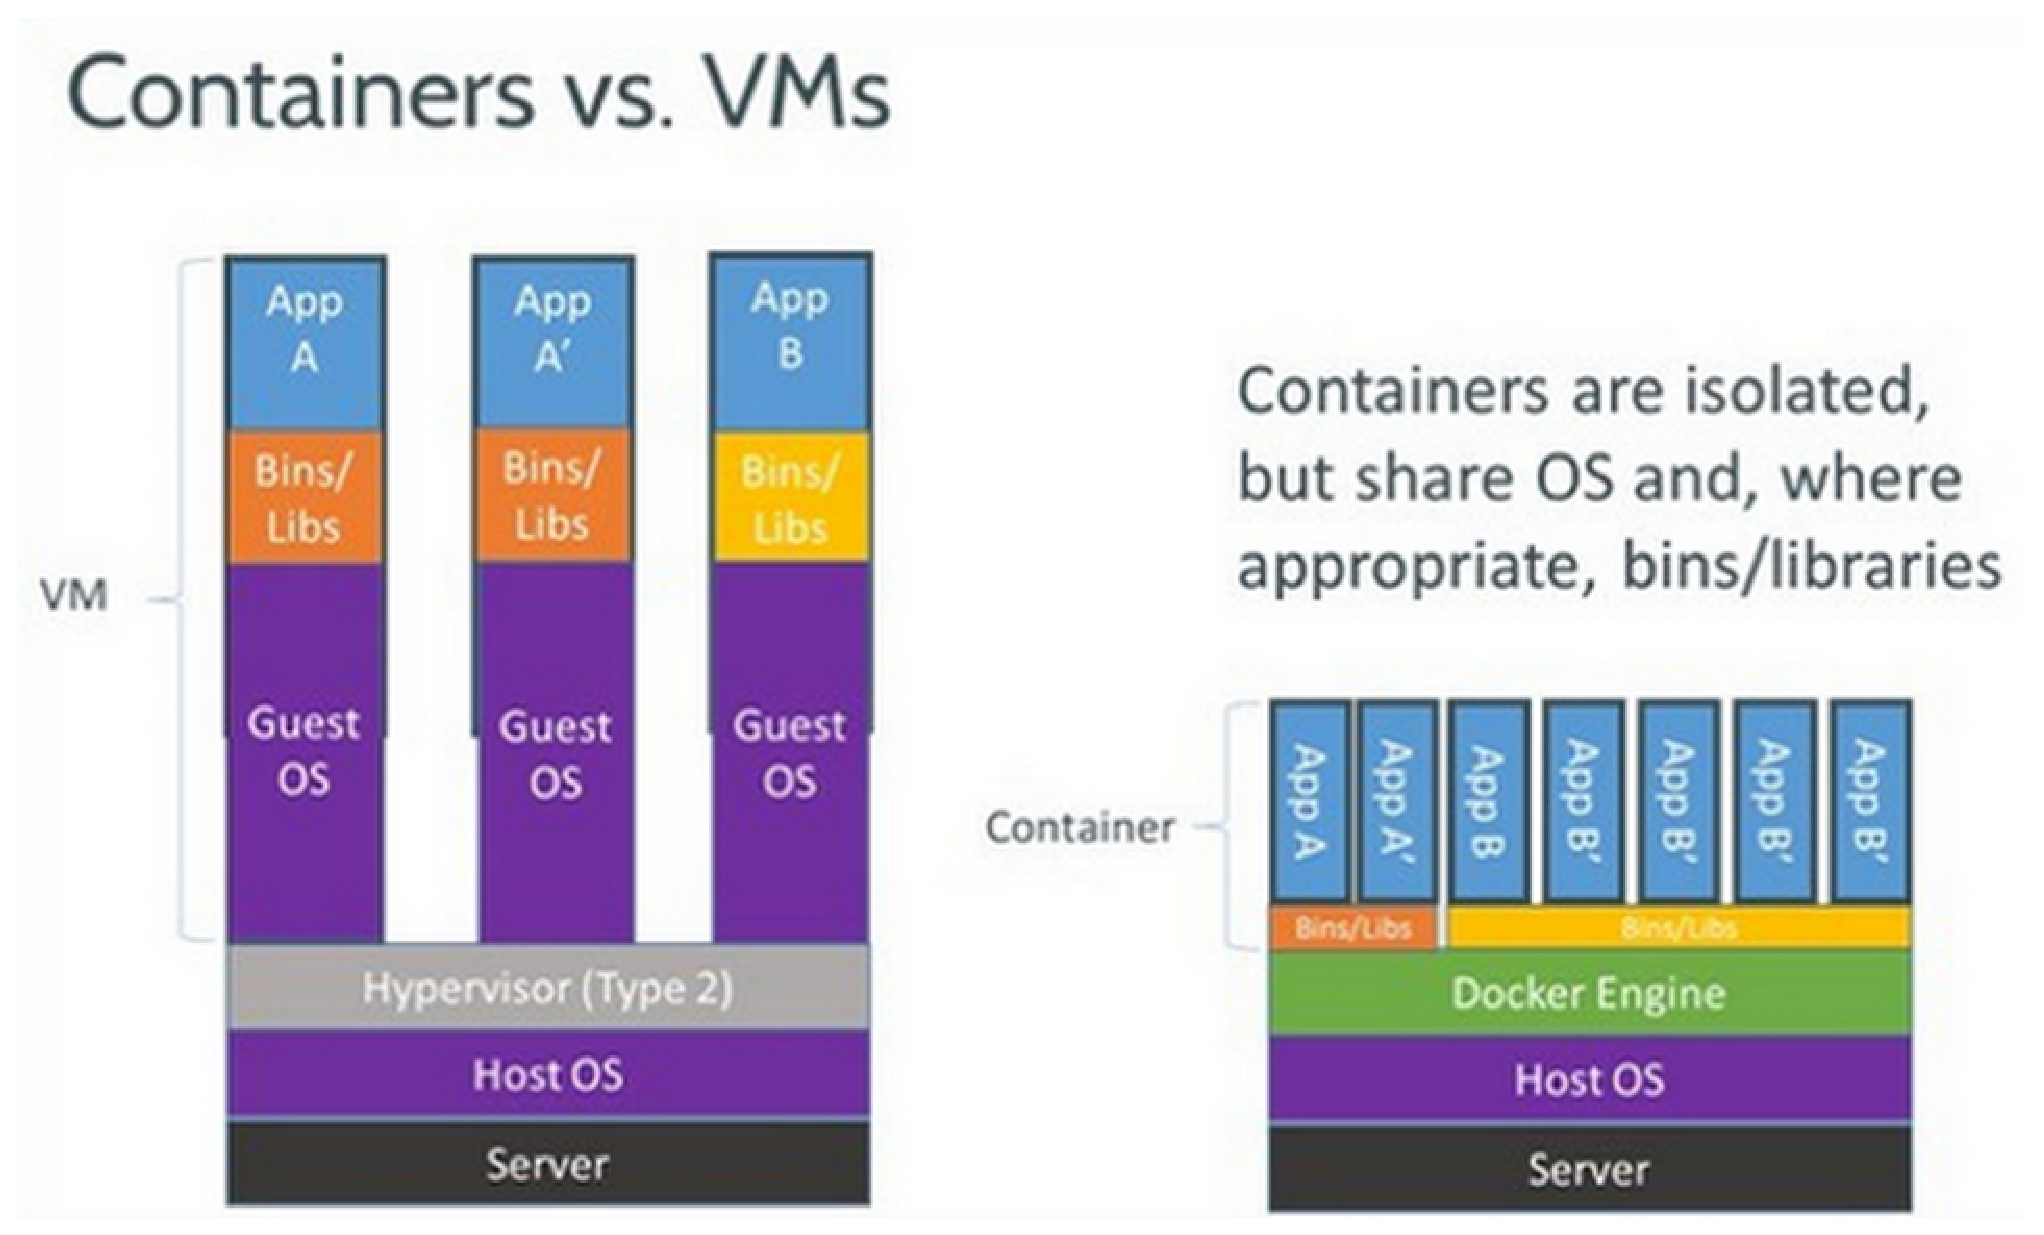
\includegraphics[height=8cm,
    angle=0]{./images/hypervisor_container.eps}}
\caption{Type-2 hypervisor with guest O/S (virtual machines) and Container}
\label{fig:hypervisor_container}
\end{figure}
 
Docker specializes in deploying apps (i.e. the container contains all needed
to run the app); while LXD specializes in deploying (Linux) Virtual Machines,
i.e. the container acts like a Linux virtual machine).

Ubuntu integrates LXD with OpenStack through its REST API; thus makes it much
closer to feature parity with real hypervisors like XEN and KVM by offering
features like snapshots and live migration. As any container technology, LXD
offers a much lower resource footprint than virtual machines:
this is, why LXD is sometimes called lightervisor.



\subsection{2011: Warden (by CloudFoundry)}

CloudFoundry started Warden in 2011, using LXC in the early stages and later
replacing it with its owncloud foundry history of containers implementation.

Warden can isolate environments on any operating system, running as a daemon and
providing an API for container management.

It developed a client-server model to manage a collection of containers across
multiple hosts, and Warden includes a service to manage cgroups, namespaces and
the process life cycle.

\subsection{2013: LMCTFY}
\label{sec:LMCTFY}

An open-source effort from Google - LMCTFY stands for “Let Me Contain That For
You”. Applications can be made “container aware,” creating and managing their
own subcontainers.

Active deployment stopped in 2015 after Google started contributing core LMCTFY
concepts to libcontainer.




\section{Requirements for container technology}



\subsection{Resource constraints:}

When you run lots of containers on a system, you do not want to have any
container monopolize the operating system, so we use resource constraints to
control things like CPU, memory, network bandwidth, etc. The Linux kernel
provides the cgroups feature, which can be configured to control the container
process resources.

\subsection{Security: }
Usually, you do not want your containers being able to attack each other or
attack the host system. We take advantage of several features of the Linux
kernel to set up security separation, such as SELinux, seccomp, capabilities,
etc.


\subsection{Isolation and Networking:}

Container processes should not have a view of any processes outside the
container. They should be on their own network. 

Container processes need to be able to bind to port 80 in different containers.

Each container needs a different view of its image, needs its own root
filesystem (rootfs). In Linux we use kernel namespaces to provide virtual
separation.

Therefore, a process that runs in a cgroup, has security settings, and runs in
namespaces can be called a container.



\section{More recent container runtimes}


Container runtime tools just modify these resource constraints, security
settings, and namespaces. Then the Linux kernel executes the processes.

After the container is launched, the container runtime can monitor PID 1 inside
the container or the container's stdin/stdout—the container runtime manages the
lifecycles of these processes.

\begin{mdframed}

Docker is often called a container runtime, but "container runtime" is an
overloaded term. When folks talk about a "container runtime," they're really
talking about higher-level tools like Docker, CRI-O, and RKT that come with
developer functionality. They are API driven.

Daemons like Docker and CRI-O, as well as command-line tools like Podman and
Buildah, should probably be called "container managers" instead.

\end{mdframed}

\verb!docker! (or to be precise \verb!dockerd!) are the tools that most people
when referring to a container runtime, i.e. launching a container image. Even if
tools for making containers (lxc) predate Docker, Docker brought containers to
the mainstream because of its simplicity.

When Docker was originally written, it launched containers using the \verb!lxc!
toolset, which predates \verb!systemd-nspawn!.

Red Hat's original work with Docker was to try to integrate libvirt
(\verb!libvirt-lxc!) into Docker as an alternative to the lxc tools, as lxc is
not available in RedHat O/S. NOTE: libvirt-lxc also did not use systemd-nspawn.
At that time, the systemd team was saying that systemd-nspawn was only a tool
for testing, not for production.

Because of all those reasons, it was decided that \verb!systemd-nspawn! should
NOT be used as a tool for launching containers.

Also, it was later decided that rather using these existing library to launch
containers, work began on \verb!libcontainer!
(Sect.\ref{sec:libcontainer-library}), as a native golang library for launching
containers. Red Hat engineering decided that this was the best path forward and
dropped libvirt-lxc.

Things have been moving very quickly over the past year, from the launch of the
App Container (appc) specification and rkt (Sect.\ref{sec:rkt-CoreOS} - 2014),
to the Open Container Initiative (OCI) - Sect.\ref{sec:OCI}), to the Cloud
Native Computing Foundation (CNCF - Sect.\ref{sec:CNCF}).


\subsection{2013: libcontainer library - Docker company}
\label{sec:libcontainer-library}
\label{sec:Docker-company}
\label{sec:Docker}

The libcontainer project was initially started by Docker company and now it has
been moved to Open Container Foundation.

\begin{mdframed}

Just as Warden did, Docker also used LXC in its initial stages and later
replaced that container manager with its own library, libcontainer, with a major
contribution from Google's LMCTFY (Sect.\ref{sec:LMCTFY}).
\end{mdframed}

\verb!libcontainer! library  uses the resource isolation features of the Linux
kernel such as cgroups and kernel namespaces, and a union-capable file system
such as aufs and others to allow independent “containers” to run within a single
Linux instance, avoiding the overhead of starting and maintaining virtual
machines.


Better than many previous systems, Docker separated itself from the pack by
offering an entire ecosystem for container management (Sect.\ref{sec:docker-command}).
\begin{verbatim}
docker [many commands]

docker image

docker container

docker build

docker run

docker push

docker pull

\end{verbatim}

A details discussion of Docker-company's \verb!docker! toolsuite is discussed in
Sect.\ref{sec:container-Docker-based}. The discussion of different commands using 
\verb!docker! is given in Sect.\ref{sec:docker-commands}.


Docker is one of the most successful open source projects in recent history,
Docker it’s fundamentally shifting the way people think about building, shipping
and running applications, smoothing the way for microservices, open source
collaboration, and DevOps.


Prior to Docker version 1.11, the Docker Engine daemon downloaded container
images, launched container processes, exposed a remote API, and acted as a log
collection daemon, all in a centralized process running as root.

Since version 1.11, the Docker daemon no longer handles the execution of
containers itself. Instead, this is now handled by containerd.

Docker is a Linux container engine, written first in Python, and later in a
programming language called Go (initially developed by Google).

Docker project was created by Solomon Hykes -- an open platform for developers
and sys admins to build, ship, and run distributed applications. This
distributed application, along with all dependency packages come as in one
package called  {\bf container}.
\footnote{\url{http://www.techrepublic.com/article/why-docker-and-why-now/}}

Docker provides the infrastructure so that a {\it container}, i.e. an excutable
image file which contains all necessarily libraries and a designated
application, can be run which will launch the desginated application on any
machine, without having to worry about installing third party libraries needed
to run that application.


Deploying a container using Docker is far simpler than OpenVZ / LXC
(Sect.\ref{sec:LXC}), so Docker-based container getting very popular. 

\begin{mdframed}
Docker is one of the most popular software that provides utilities and
environment, that provides the capability to create a Docker-based image file,
establish a (Docker-based) container from that image, and run on an isolate
memory space, on an existing host operating system.
 
Docker helps you create a reproducible environment. You are able to specify the
specific OS, the exact version of different libraries, different environment
variables and their values among other things. Most importantly you are able to
run your application in isolation inside of that environment.


Docker containers run the host’s Linux kernel. Docker is about isolation, not
about virtualization. The advantage is that a Docker image does not contain an
operating system! So, a container (e.g. Docker image) does not boot Windows, or
Linux, it enabls an app running on the existing kernel of the host, but in an
isolate environment with dedicated installed dependency software packages.
So it starts up in milliseconds as oposed VirtualBox in maybe 45 seconds. I can
run hundreds of containers on my Laptop.


%\section{Container-based virtualization (OS-level virtualization) vs. Hypervisor-based virtualization}
% {Cloud O/S running on Linux containers vs.
% Traditional VM running on hypervisor}


Docker uses a so-called layered file system which enables the containers to
share common parts and the end result is that containers are way less of
resource-hog on the host system than a virtual machine.


\end{mdframed}

\textcolor{red}{In Docker 0.8, Docker is not a replacement for LXC as Docker
still uses LCX, i.e. LXC provides low-level capabilities of the O/S kernel.
Since Docker 0.9, it uses a new driver, libcontainer, which does not use LXC at
all to create containers, but uses cgroups/namespaces directly}. 

Docker offers a high-level tool with several powerful functionalities:

\begin{enumerate}
  \item Docker defines a format for bundling an application and all its
  dependencies into a single object which can be transferred to any
  docker-enabled machine.
  
  The object is  executed there with the guarantee that the execution
  environment exposed to the application will be the same. To allow the
  container to run the app the same everywhere, Docker use LXC to create the
  minimal requirement for an operating system in the container. Hence, the
  container needs to have a filesystem, and Docker uses AuFS - a {\bf a layered
  filesystem}  so you can have a read only part, and a write part, and merge
  those together. So a container is like a light-weight O/S with an integrated
  application. The size of a container can be 1GB in size.
  
  \item Application-centric rather than machine-centric:
  
\end{enumerate}

A full virtualized system gets its own set of resources allocated to it, and
does minimal sharing. You get more isolation, but it is much heavier (requires
more resources). With LXC you get less isolation, but they are more lightweight
and require less resources. So you could easily run 1000's on a host, and it
doesn't even blink.



\subsection{specification: App Container (AppC) specification}
\label{sec:AppC-specification}

App Container (appc) specification is an open specification that defines several
aspects of how to run applications in containers: an image format, runtime
environment, and discovery protocol.

CoreOS, one of the original minimalized Linux systems, announced at its
inaugural annual conference the formal entry of Google, VMware, Red Hat, and
hybrid cloud OS maker Apcera into a gathering coalition of industry partners
backing App Container, or appc, the specification developed by CoreOS for its
Rocket runtime system.

The coallication:
\begin{verbatim}
Google
CoreOS

VMware: support of appc in its own minimalized Linux, called Project Photon


CoreOS has announced it is receiving a Red Hat senior engineer and a major
Docker contributor, Vincent Batts, as that company’s maintainer of appc.

Batts will join Google’s Tim Hockin (another Docker maintainer) and Twitter’s
Charles D. Aylward.
\end{verbatim}

\begin{itemize}
  
  \item  Apcera will premiere this week its own appc implementation, named
  Kurma, which at this early stage is being described as 'an execution
  environment for running applications in containers.'
  
  \item \verb!rkt! is CoreOS's implementation of appC specification.
  
  Quay.io, the private, secure Docker repository host it acquired last August
  and the foundation of its CoreOS Enterprise Registry (Sect.\ref{sec:Quay.IO}),
  to act as a secure repository for rkt images as well as Docker.
  
  Docker’s runtime currently uses Docker Hub as its centralized distribution
  center by default, although the image name may specify another location. Polvi
  explains to us that \verb!appc!, by comparison, is more like git: decentralized by
  default.
  
\end{itemize}

\url{https://thenewstack.io/coalition-for-app-container-spec-shows-docker-is-not-the-standard-for-everyone/}

\url{https://coreos.com/rkt/docs/latest/app-container.html}

\subsection{-- 2014: rkt - CoreOS's Rocket}
\label{sec:rkt-CoreOS}

Rocket started by CoreOS released reference implementation of an open Rocket
specification - appC (Sect.\ref{sec:AppC-specification}), standardizing the
packaging of images and runtime environments for Linux containers.

CoreOS Rocket (rkt) is the first credible challenger to Docker's dominance in
the container space. Simply put, rkt is a more secure container technology,
designed to alleviate many of the flaws inherent in Docker's container model.

\begin{verbatim}

“From a security and composability perspective, the Docker process model – where
everything runs through a central daemon – is fundamentally flawed. To ‘fix’
Docker would essentially mean a rewrite of the project, while inheriting all the
baggage of the existing implementation.”

\end{verbatim}

NOTE: It's worth noting that Docker has since remediated some of its more
critical security flaws—for example, its 1.10 release eliminated the need of
running containers as root, addressing a longstanding security gripe among its
adopters.
\url{https://www.upguard.com/articles/docker-vs-coreos}

\url{https://www.redhat.com/en/blog/rkt-appc-and-docker-take-linux-container-upstream}

\subsection{2015: Open Container Initiative (OCI)}
\label{sec:OCI}

Traditional namespace-separated containers were popular, but people also had the
desire for virtual machine-level isolation.

Because of that, the Open Container Initiative (OCI) was formed in June 2015,
party because people wanted to be able to launch containers in additional ways.

The idea behind OCI was to take the widely deployed runtime and image format
implementation from docker and build an open standard in the spirit of appc

\begin{verbatim}

Creating and maintaining formal specifications ("OCI Specifications") for
container image formats and runtime, which will allow a compliant container to
be portable across all major, compliant operating systems and platforms without
artificial technical barriers.

\end{verbatim}

Intel and Hyper.sh were working on KVM-separated containers, and Microsoft was
working on Windows-based containers.

The OCI wanted a standard specification defining what a container is, so the OCI
Runtime Specification was born.


The OCI Runtime Specification defines a JSON file format that describes what
binary should be run, how it should be contained, and the location of the rootfs
of the container. Tools can generate this JSON file.
Then other tools can read this JSON file and execute a container on the rootfs.

NOTE: The libcontainer parts of Docker were broken out and donated to the OCI.


\subsection{-- runC implementation}


runC is a new frontend tool to read the OCI Runtime Specification JSON file and
interact with libcontainer to run the container.
 
Sect.\ref{sec:runC-utility}


\subsection{-- other implementations: RailCar (Oracle), Kata (runV + Clear Container)}
\label{sec:RailCar}
\label{sec:runV}
\label{sec:Kata-containers}

Both Clear Containers and Hyper.sh's runV tools were created to use the OCI
Runtime Specification to execute {\it KVM-based containers}, and they are
combining their efforts in a new project called Kata.

Last year, Oracle created a demonstration version of an OCI runtime tool called
RailCar, written in Rust.

NOTE: CRI-O (Sect.\ref{sec:CRI-O}) supports launching containers via these tools.

Vincent Batts worked on adding a tool, \verb!nspawn-oci!, that interpreted an OCI
Runtime Specification file and launched systemd-nspawn, but no one really picked
up on it, and it was not a native implementation.

There is currently no effort to implement
\begin{verbatim}
systemd-nspawn --oci OCI-SPEC.json
\end{verbatim}
If and and if it is to be  accepted by the systemd team for support, then CRI-O, Docker, and
eventually Podman would be able to use it in addition to runc and Clear
Container/runV.

INTERESTING ARTICLE by Daniel Walsh 
\url{https://opensource.com/article/18/1/history-low-level-container-runtimes?source=post_page---------------------------}



\subsection{2016: Windows Container}

Microsoft add container support Microsoft Containers to the Microsoft Windows Server
operating system in 2015 for Windows based applications, called Windows
Containers.

Recently, Microsoft announced the general availability of Windows Server 2016,
and with it, Docker engine running containers natively on Windows.
With this implementation Docker is able to run Docker containers on Windows
natively without having to run a virtual machine to run Docker (earlier Docker
ran on Windows using a Linux VM).

\url{https://blog.docker.com/2016/09/build-your-first-docker-windows-server-container/}

\subsection{Cloud Native Computing Foundation (CNCF)}
\label{sec:CNCF}

A cloud-native app allows IT and software to move faster. 

CNCF was created to help finding the standard/technologies that enable cloud
portability without vendor lock-in of cloud-native apps. Projects that falls into CNCF are
\begin{enumerate}
  \item Kubernetes
  
  \item Prometheus, and Envoy
  
  \item containerd
  
  \item \ldots
\end{enumerate}


The Linux Foundation is the parent of CNCF. We are one of the LF’s largest sub-foundations


\subsection{2014 - Kubernetes (K8s) and CRI interface}
\label{sec:Kubernetes}
\label{sec:K8s}
\label{sec:CRI-interface}

Kubernetes is a system for orchestrating containers, i.e. launching and manage
them, regardless of where (cloud-specific vendor) the containers run.

Developped at Google, Kubernetes originally leveraged Docker for running
containers, and Docker is still the default container runtime today.

Later, CoreOS offered a bunch of patches to kubernetes to use Rkt as an
alternative to Docker (Sect.\ref{sec:rkt-CoreOS}).
Then, upstream Kubernetes saw this as a problem as they did not want to have to modify
the kubernetes code base for each new container runtime.
Upstream kubernetes decided to create an API to define calls that it would make
into container runtimes, i.e. the container runtimes (like Rkt or Docker CLI) must provides. 

This set of APIs is standardized as the Container Runtime Interface (CRI).
The first container runtime to support this is CRI-O (Sect.\ref{sec:CRI-O}).

This means anyone can create his own container runtime and simply have it speak
the CRI interface in order to run containers under kubernetes.
\begin{itemize}
  
  \item CRI-O, which was the first container runtime created for the kubernetes
  CRI interface
  
  \item rkt runtime - dropped the support
  
  \item cri-containerd - Sect.\ref{sec:cri-containerd}
  
  NOTE: Containerd (Sect.\ref{sec:containerd}) isn’t implementing the CRI
  interface, it does so with another daemon called \verb!cri-containerd! which acts as
  a shim between containerd itself and the kubelet.

  Docker CLI has since broken out many of its features into containerd and now
  supports CRI through \verb!containerd! as well.
  
  \item dockershim - Sect.\ref{sec:dockershim}
  
If the container runtime of choice is Docker, it is used through the built-in
\verb!dockershim! CRI implementation inside of the kubelet.

  \item fratki - Sec.\ref{sec:fratki}
\end{itemize}


Kubernetes is an open source container orchestration platform, allowing large
numbers of containers to work together in harmony, reducing operational burden.

\begin{itemize}
  \item   Running containers across many different machines
  \item   Scaling up or down by adding or removing containers when demand changes
  \item   Keeping storage consistent with multiple instances of an application
  \item   Distributing load between the containers
  \item   Launching new containers on different machines if something fails

\end{itemize}

Under the hood, Kubernetes can integrate with the Docker engine to coordinate
the scheduling and execution of Docker containers on Kubelets (Sect.\ref{sec:Kubernetes-details}).


\url{https://www.cncf.io/blog/2019/06/06/reflections-on-the-fifth-anniversary-of-kubernetes/}

\subsection{-- containerd}

Sect.\ref{sec:containerd}


\subsection{2015: RedHat OpenShift}
\label{sec:OpenShift}

OpenShift and Docker both use kernel isolation features to keep tenant processes separate.
Both use cgroups to limit the CPU, memory, and IO of tenants.

For Docker that is primarily through LXC and for OpenShift that is largely
through SELinux and Multiple Category Security (MCS).

Docker uses AUFS for advanced disk and file copy-on-write sharing, OpenShift
neither requires nor is incompatible with such a system.

Inside the container, OpenShift models units of functionality (web servers, dbs)
via "cartridges", which are a set of shell script hooks that are called when the
system is invoked. The API is described here. A cartridge is roughly similar to a docker image.
\url{https://github.com/openshift/origin-server/blob/master/documentation/oo_cartridge_developers_guide.adoc}

As of June 2015, OpenShift Origin 1.0 runs on top of Docker and Kubernetes, and
you can build and develop multi container apps that run on the Docker runtime.
OpenShift adds build, image workflow and promotion, and secure container cluster
operations on top of Kube and Docker

\url{https://stackoverflow.com/questions/16840342/how-does-docker-compare-to-openshift}

\subsection{2017+: container management tools become mature}

Hundreds of tools have been developed to make container management easier.


Kubernetes; since its adoption into the Cloud Native Computing Foundation (CNCF)
in 2016, VMWare, Azure, AWS, and even Docker have announced their support, on
top of their infrastructures.

\begin{enumerate}
  \item   Ceph and REX-Ray set standards for container storage, 
  \item while Flannel connects millions of containers across datacenters. 
  
  \item And in CI/CD, Jenkins is completely changing the way we build and deploy apps.
  
\end{enumerate}

\url{https://blog.aquasec.com/a-brief-history-of-containers-from-1970s-chroot-to-docker-2016}


Docker, the company, cannot monetize upon the technology, because the moment
they start charging for their containerization technology, people will switch to
an alternative container technology, especially now that Kubernetes has won the
orchestration "wars" and made it so easy to switch the underlying technology.

Docker doesn’t do anything you can’t do with lxc tooling and an object store
(registry).

For example, GitHub does not charge for git, but instead for the convenient
layers that they add on top of it.
Google does not charge for Kubernetes but you can buy support which every
enterprise company wants and since GKE happens to be the most convenient way to
get a K8s cluster rolling in the cloud (for most circumstances) and also now on
a box now with GKE On-Prem, many will choose that path so Google still gets
their money, just from product / services / support on top of the free core.


\section{Image vs. Container}
\label{sec:Docker-image}

As any program that runs, it becomes a process and exist within a memory space
with a given root file system, from that information about libraries, path to
file/folder can be retrieved.

A {\bf container} provides a sandbox environment within it a process can run.
The information about this sandbox is kept in an {\bf image} which is a binary
file that can be created from a text file named Dockerfile
(Sect.\ref{sec:Dockerfile-tutorial}).

You can think of a container like running a virtual machine, without the
overhead of spinning up an entire operating system.

With new features provided by recent Linux kernel
(Sect.\ref{sec:container-technology-history}), a running process of a container
can have its own incremental files system, where layers are reused across
containers. In addition, every container has its own network stack, therefore
its own IP-address, and its own process space.

The software that runs inside a container is usually designed as a single
purpose application; but nowadays we can put a complete bootable operating
system inside a container, thanks to the development of Docker - a set of
user-friendly tools that enables the creation of images, launching container
from an image, manages the container + images.
 
A container is launched by runing an {\it image} - a file  that includes
everything needed to run an application-the code, a runtime, libraries,
environment variables, and configuration files.

A {\bf container} provide a sandbox environment for running the cloud O/S better
than running on traditional VM on hypervisor. {\bf Container-based
virtualization} is a virtualization method that uses a single kernel to run
multiple containers, each container is hosted on a single cloud O/S.
\url{http://searchservervirtualization.techtarget.com/definition/container-based-virtualization-operating-system-level-virtualization}

Containers was designed to allows the host O/S kernel to support all of the
resource-isolation use cases, without the overhead and complexity of running
multiple kernel instances as the case of using hypervisor.
\url{http://lwn.net/Articles/528078/}

A disadvantage of container-based virtualization, however, is that the container
runs using the same operating system that the host uses.
\url{http://searchservervirtualization.techtarget.com/tip/Making-the-case-for-container-based-virtualization-over-hypervisors}

\section{What is a container? and how many types of them?}
\label{sec:containers_Linux}


So, a {\bf container} is like a virtual environment, in that a software can
run in isolation of other software running on the physical host machine.
There is no spec specifying what a container should implement.

To achieve creating a sandbox, Docker container's default \verb!union!
\verb!filesystem! layer and files written to volumes is: container's union
filesystem layer data is always lost when removing the container.

There are several Linux-based Containers projects,
Sect.\ref{sec:container-technology-history}. At their core, containers provide a
sandbox environment [complete enough for a program to run].
So, it provides a portable way of packaging software. What makes them special is
that when you run a container, you know exactly how it will run - it’s
predictable, repeatable and immutable.
There are no unexpected errors when you move it to a new machine, or between
environments. All of your application’s code, libraries, and dependencies are
packed together in the container as an immutable artifact.

The container technology is not new, but is getting so popular recently
primarily because kernel support is now available in Linux (namespace and
cgroups) kernel 3.8 (Feb 2013).

To run a container, we need a container runtime engine or daemon.
Most people when referring to a container runtime think of Docker
(Sect.\ref{sec:Docker}). Even if tools for making containers (lxc) predate
Docker, Docker brought containers to the mainstream because of its simplicity.


\label{sec:OCI-runtime}
The Open Container Initiative (OCI) is a Linux Foundation project to design open
standards for operating-system-level virtualization, most importantly Linux
containers. OCI develops runC (Sect.\ref{sec:runC-utility}).
OCI has two specs, a Image spec and a Runtime spec.

The OCI Runtime Specification outlines how to run a containers “filesystem
bundle” that is unpacked on disk. At a high-level an OCI implementation would
download an OCI Image (OCI Image Specification) then unpack that image into an
OCI Runtime filesystem bundle. At this point the OCI Runtime Bundle would be run
by an OCI Runtime. 

When we talk about container, it can be confusing, as it can refers to a format
or a software that manage files in that format
(Sect.\ref{sec:container-Docker-based}). 

It’s important to distinguish Linux containers, e.g. created using \verb!docker!
utility (Sect.\ref{sec:Docker}), from traditional and more common type 1 or type
2 hypervisors.



\verb!containerd! (Sect.\ref{sec:containerd} - from Docker company, and is a
project within CNCF - Sect.\ref{sec:CNCF}) fully leverages the OCI runtime
specification (Sect.\ref{sec:OCI-runtime}). Because of its massive adoption,
containerd is the industry standard for implementing OCI. It is currently
available for Linux and Windows.

 
When it comes to containers there are a ton of APIs in the ecosystem.
This means that users have had to think about all of the different APIs, but consolidation is coming

Example:  In Kubernetes environment
\begin{verbatim}
# how a container gets created in a Kubernetes environment. 
 
 
Orchestration API -> Container Engine API -> Kernel API

# digging a deeper level

Kubernetes Master -> Kubelet -> Docker Engine -> containerd -> runc -> Linux kernel


# in the future, this may become
Kubernetes Master -> Kubelet -> containerd -> runc -> Linux kernel


\end{verbatim}
Example: In OpenShift platform
\begin{verbatim}

Kubernetes Master -> Kubelet -> CRI-O -> runc -> Linux kernel

\end{verbatim}

But the most important layer, and the one where most end users should be focused
on is the Kubernetes Master API. This is where they should learn, integrate, and
focus investment. This is the layer that will help users move faster, deploy
apps better, etc.


Now, we compare between CRI-O and \verb!containerd! (Sect.\ref{sec:CRI-O})




SUMMARY: With LXC and AuFS you can share the bulk of the 1GB and if you have
1000 containers you still might only have a little over 1GB of space for the
containers OS, assuming they are all running the same OS image.   
\url{http://stackoverflow.com/questions/16047306/how-is-docker-io-different-from-a-normal-virtual-machine}

Docker also introduces DockerFile, lightweight "configuration as code", that
makes it easy to share containers (or at least container definition) -
Sect.\ref{sec:Dockerfile-tutorial}.
Also, docker index offers a simple way to distribute ready-to-deploy container
images. \url{https://groups.google.com/forum/\#!topic/docker-user/rS_u1bkhXoI}

\url{http://stackoverflow.com/questions/17989306/what-does-docker-add-to-just-plain-lxc}

\subsection{Container image format}

The format of a Docker-based image is not covered in details here. However, it's
important to know that this file can be created using the information  given
from a text file called {\bf Dockerfile} (Sect.\ref{sec:Dockerfile-tutorial}).
Dockerfiles define a build process, which, when fed to the ‘docker build’
command, will produce an {\bf immutable} docker image.

You can think of this as a snapshot of your application, ready to be brought to
life at any time.


\begin{enumerate}
  \item Docker-format:
  
  
  The Docker engine itself is responsible for running the actual container image built by running ‘docker build’. 
  
  
  \item Pod: 
  
  A Pod encapsulates an application container (or, in some cases, multiple
  containers), storage resources, a unique network IP, and options that govern
  how the container(s) should run.
  
  A Pod is the basic building block of Kubernetes–the smallest and simplest unit
  in the Kubernetes object model that you create or deploy. A Pod represents a
  running process on your cluster.
  
  
\end{enumerate}

\subsection{CRI-O}
\label{sec:CRI-O}


CRI is the Container Runtime Interface defined by kubernetes to allows for
pluggable container runtime for k8s (Sect.\ref{sec:Kubernetes}).

There are currently several implementations, among them are
\verb!cri-containerd! and \verb!cri-o!, both are actually end up use
\verb!oci/runc! as the low-level tool to launch a container on the host O/S
(Sect.\ref{sec:runC-utility}).

CRI-O leverages all of the OCI standards
\begin{verbatim}

Runs containers using the OCI Runtime tools defaulting to runc.

Managing container images following the OCI image specification.

Uses the OCI-Runtime-tools for generating the OCI Runtime Specification

CNI for setting up the container networking.

containers/image for pulling container images from container registries like docker.io

\end{verbatim}

Besides support using runC, similar to what Docker can do, in addition to that
CRI-O has support for running containers using virtualization technologies like
Clear Containers, and soon Kata Containers (Sect.\ref{sec:Kata-containers}).

At the time of this writing, there are mainly 4 containers runtimes implementing
the CRI interface: CRI-O, fratki (Sect.\ref{sec:fratki}), cri-containerd, dockershim.


CRI-O gives OpenShift users the ability to pull and run standard container
images based on the OCI specifications (Distribution, Image, and Runtime).


\url{https://medium.com/cri-o/container-runtimes-clarity-342b62172dc3}


\subsection{Container software}

\chapter{Docker company}

\section{docker utility}


In 2016 the container space was booming and Docker company decided to split the monolith
tool \verb!docker! into separate parts, some of which other projects can even
build on — that’s how \verb!containerd! happened. In an effort to make Docker Engine
smaller, better, faster, stronger, Docker is spli into different components,
i.e. break out into separate projects
\begin{enumerate}
  \item  \verb!runc!:  the standalone runtime for the component as the Docker runtime for managing containers.
  
  \item \verb!containerd!:  the container supervision out of the core Docker Engine and into a separate daemon. 
  
  It enables adding runc to the stack as well as managing 100s of containers.
   This allows users to replace the runc binary on their system with an
   alternate runtime and get the benefits of still using Docker’s API.
  
  \item \verb!docker-cli!: 
\end{enumerate}

\begin{verbatim}
ps fxa | grep docker -A 3  

\end{verbatim}
dockerd is started and containerd is running as a child process too. Like described, dockerd needs containerd 

NOTE: We do not see runc in the chain, we know containerd-shim takes over after runc has started the container. 
\begin{verbatim}
dockerd --> containerd --> containerd-shim --> "sleep 60" (desired process in the container).


\end{verbatim}

\subsection{List of all commands}
\label{sec:docker-commands}

\begin{verbatim}
docker run – Runs a command in a new container.
docker start – Starts one or more stopped containers
docker stop – Stops one or more running containers
docker build – Builds an image form a Docker file
docker pull – Pulls an image or a repository from a registry
docker push – Pushes an image or a repository to a registry
docker export – Exports a container’s filesystem as a tar archive
docker exec – Runs a command in a run-time container
docker search – Searches the Docker Hub for images
docker attach – Attaches to a running container
docker commit – Creates a new image from a container’s changes
\end{verbatim}

\subsection{docker image: examine the local images}
\label{sec:docker-image-command}

//NOTE: list local images can be done either using
\begin{verbatim}
docker images 

docker image ls
\end{verbatim}
An image is uniquely identified by its HASH code (or IMAGE ID), which is showed
via the above commands.


Example: show all information about images (REPOSITORY, TAG, IMAGE-ID, WHEN-created, SIZE)
\begin{verbatim}
REPOSITORY                     TAG                         IMAGE ID            CREATED             SIZE
mgs_baseimage                  latest                      430692be693d        7 days ago          1.02GB
nvidia/cuda                    9.0-devel-ubuntu16.04       45621eed160b        4 weeks ago         2.08GB
\end{verbatim}


Example: show only REPOSITORY name and TAG 
\begin{verbatim}
docker images --format "{{.Repository}}:{{.Tag}}"


mgs_baseimage_cuda10:latest
mgs_baseimage:latest
nvidia/cuda:10.0-devel-ubuntu16.04
nvidia/cuda:9.0-base
nvidia/cuda:9.0-devel-ubuntu16.04
nvidia/cuda:9.0-runtime-ubuntu16.04

\end{verbatim}


\begin{enumerate}
  \item working with images - Sect.\ref{sec:Docker-image}
  \item remove image - Sect.\ref{sec:docker-rmi}
\end{enumerate}


\begin{verbatim}

docker image [subcommands]


// list all available local images
docker image ls

// build an image from 'Dockerfile'
docker image build [-f Dockerfile]


docker image history 
\end{verbatim}

\subsection{-- update an image}

An image is non-modifiable. If you want to add a new layer, i.e. install
somethings, a new image (and optinally, the tag) has to be created.

Suppose you run an image, i.e. having a container ID
\begin{verbatim}
docker run -it <image-name>  
\end{verbatim}


Inside the container, as 'root', you just install packages if you need.


While the command is running, detach from the container using Ctrl-p + Ctrl-q keys 

Then you save the state of the given container to an image
\begin{verbatim}
docker commit <CONTAINER_ID>   <IMAGE_NAME:TAG>

docker commit 5976e4ae287c ubuntu-nginx
\end{verbatim}


Finally, you can attach again
\begin{verbatim}
docker attach <CONTAINER_ID>
\end{verbatim}

\subsection{-- remove an image}

Sect.\ref{sec:docker-rmi}

\subsection{docker run: launch a container from an image}
\label{sec:docker-run-command}

Check Sect.\ref{sec:Docker-run}.


There are two options: 
\begin{enumerate}
  \item bake the binary-app inside the Docker image
  
  \item separate the binary-app from the Docker image (only contains runtime environment)
\end{enumerate}


Remember that you uses either CMD command or ENTRYPOINT command (or both) from Dockerfile.
In that you have two forms: \verb!shell! form and \verb!exec! form (Sect.\ref{sec:Dockerfile-CMD}).


\subsection{-- option 1 (binary-app inside Docker image)}

Example: the argument are also fixed (i.e. \verb!"hello"!), and the binary app is inside
\verb!/bin/echo! the image.
\begin{verbatim}
FROM ubuntu
COPY ./binary_app /bin/
ENTRYPOINT ["/bin/binary_app"]
CMD ["hello"]
\end{verbatim}

\subsection{-- option 2 (binary-app outside Docker image or argument is a file on host)}


We need to inject the volume: use Docker volumes to inject files from your host
machine to the container when running it.

\begin{verbatim}
docker run -v /local/path/to/file1:/container/path/to/file.txt -t boot:latest python boot.py file1.txt
\end{verbatim}
NOTE: Then /local/path/to/file1 would be the path on your host machine which will override 
/container/path/to/file.txt on the container.

\subsection{-- option 3 (argument is a file on host)}


OPTION 1: may also make your script read from STDIN and then pass data to docker using cat, and run the docker image in interactive mode 
(\verb!-i! option)
\begin{verbatim}
cat /path/to/file | docker run -i --rm boot python boot.py
\end{verbatim}


OPTION 2:
We need to inject the volume: use Docker volumes to inject files from your host
machine to the container when running it.

\begin{verbatim}
docker run -v /local/path/to/file1:/container/path/to/file.txt -t boot:latest python boot.py file1.txt
\end{verbatim}
NOTE: Then /local/path/to/file1 would be the path on your host machine which will override 
/container/path/to/file.txt on the container.



As a docker just provide an isolated environment, with all necessary packages, 
typically we use the Docker container (as a sandbox) to launch  your program of interest
\begin{verbatim}
docker run <IMAGE-NAME>  <program to run>

# if the <program> is already part of the image
docker run <image-name>


# just create the container, but does not run
docker run -d <image-ID> 

# run a stopped or freshly created container
docker start -ai mad_brattain


\end{verbatim}

Docker engine looks for local image with given name
\begin{itemize}
  \item if yes: instantiate a container from information in that image
  \item if no: download that image from a given Docker registry (e.g. Docker Hub) first, and continue the above steps
\end{itemize}
NOTE: Sect.\ref{sec:Docker-image} explains how to check for local images.


Right after that command, the terminal put you into {\bf attached mode} or {\bf
foreground mode} of the container, i.e. you see output from the container to the
console, but you can not interact with the terminal, until the container
complete, and exit. If you press Ctrl-C, it terminates the container, and you
get back your terminal, but of course there is no container running if you check
with either
\begin{verbatim}
docker container ls

docker ps
\end{verbatim}



\textcolor{red}{Run in detached mode}: The container immediately run in
background, and you get back the terminal for continuing your work. It will
display a HASH code that uniquely refers to that running container.

\begin{verbatim}
docker run -d alpine sleep 60  

docker run -d jenkins
\end{verbatim}

\textcolor{red}{When the container ends?} It ends when the command given to CMD
statement finishes. If you want your container to remain active, you have to
ensure that your CMD keeps running.


Example: launch a container, using the image stored from 
\verb!https://hub.docker.com/r/docker/whalesay! URL 

\label{sec:docker/whalesay}
The docker/whalesay image is a Ubuntu distro with a custom build of the cowsay
program that displays Docker’s whale instead of the usual cow.

\begin{verbatim}
docker run docker/whalesay cowsay boo
\end{verbatim}

\begin{verbatim}
FROM ubuntu:14.04

# install cowsay, and move the "default.cow" out of the way so we can overwrite it with "docker.cow"
RUN apt-get update && apt-get install -y cowsay --no-install-recommends && rm -rf /var/lib/apt/lists/* \
    && mv /usr/share/cowsay/cows/default.cow /usr/share/cowsay/cows/orig-default.cow

# "cowsay" installs to /usr/games
ENV PATH $PATH:/usr/games

COPY docker.cow /usr/share/cowsay/cows/
RUN ln -sv /usr/share/cowsay/cows/docker.cow /usr/share/cowsay/cows/default.cow

CMD ["cowsay"]
\end{verbatim}



Example: just open a shell, and map the host's port 81 to container's port 80
\begin{verbatim}

docker run -it -p 81:80 ubuntu-nginx /bin/bash

//inside the container, run the daemon, e.g.
root@....:  nginx&

//detach the container [Ctrl-p + Ctrl-q]

// and on any remote machine, with IP to the machine hosting the container,
// open the browser, type IP of that machine and port 81 

\end{verbatim}

\textcolor{red}{Testing:} the image is downloaded (from Docker Hub)
\begin{verbatim}
docker run hello-world
\end{verbatim}


\begin{verbatim}
To generate this message, Docker took the following steps:
 1. The Docker client contacted the Docker daemon.
 2. The Docker daemon pulled the "hello-world" image from the Docker Hub.
 3. The Docker daemon created a new container from that image which runs the
    executable that produces the output you are currently reading.
 4. The Docker daemon streamed that output to the Docker client, which sent it
    to your terminal.
\end{verbatim}

After an image has been downloaded, you can then run a container using the
downloaded image with the run subcommand.


Check the list of all available container (images)
\begin{verbatim}
docker image ls

docker images
\end{verbatim}


Run:
\begin{verbatim}
docker run <container-file-name>

//example
docker run hello-world

// run the 'bash' command on the 'ubuntu' container 
//  and keep it persistent with '-i -t' options
docker run -it ubuntu bash


// run the container and map machine's port 4000 to container's port 80
docker run -p 4000:80 friendlyhello
 
   //run as a daemon (-d option)
docker run -d -p 4000:80 friendlyhello 
\end{verbatim}

\subsection{-- status of a container}

A container can be in one of the following status
\begin{enumerate}
  \item \verb!created!: (freshly) created, but not run yet

Freshly created container
\begin{verbatim}
docker create [OPTIONS] IMAGE [COMMAND] [ARG...]
\end{verbatim}
creates a writeable container layer over the specified image and prepares it for
running the specified command. The container ID is then printed to STDOUT.

Option \verb!-d! allows us to create a container from an image but never run it
\begin{verbatim}
docker run -d 
\end{verbatim}
which you can start later with
\begin{verbatim}
docker start <container_id> 
\end{verbatim}

  \item \verb!exited!: completed the program associated with the container
  
  \item \verb!stopped!: a running is stopped by the \verb!docker stop! command

\begin{verbatim}
docker stop CONTAINER_ID
\end{verbatim}
you can relaunch the same container with the command 
\begin{verbatim}
docker start CONTAINER_ID
\end{verbatim}, and the data and settings will be the same.

\end{enumerate}

\subsection{-- docker run: open an interactive shell}



Suppose you want to open a bash shell, instead of running the program as indicated in 'CMD'
command
 
\begin{verbatim}

sudo docker run -it --entrypoint=/bin/bash <imagename>
\end{verbatim}

\subsection{-- docker run: as non-root user}

docker run gives us a way to do this: the --user parameter.

Sect.\ref{sec:docker-volume}

To get the exact user on the host, we pass the result to the \verb!-u! parameter.

\begin{verbatim}
docker run --user <username> <docker-image>
 
docker run -it -u `id -u $USER` debian:jessie /bin/bash
\end{verbatim}

\subsection{-- privilege: CPU/memory maximum usage}


By default, all containers are created equal; they all get the same proportion
of CPU cycles and block IO, and they could use as much memory as they need.

\begin{verbatim}
$ docker run -it -m 4m ubuntu:14.04 bash

$ docker run  -m 4m ubuntu:14.04 python3 -c 'open("/dev/zero").read(5*1024*1024)'
\end{verbatim}

\subsection{docker start: run a container from a stopped/freshly created container}
\label{sec:docker-start}

Run is a combination of create and start. It creates the container and starts it.
\begin{verbatim}
docker run [...] = docker pull [...] + docker start [...]
\end{verbatim}

Start will start any stopped containers. This includes freshly created containers.



\subsection{docker build: create a local image from an existing image}
\label{sec:docker-build}

We discuss the \verb!docker build! command, as part of Docker package (Sect.\ref{sec:Docker}).

Example: Dockerfile that create an image, using the base as \verb!docker/whalesay! image.

This tells Docker to use the latest tag of the docker/whalesay image, install
the fortune program via apt-get, and execute cowsay feeding it with the output
of fortune.

\begin{verbatim}
# Dockerfile file
FROM docker/whalesay:latest
RUN apt-get -y update && apt-get install -y fortunes
CMD /usr/games/fortune -a | cowsay
\end{verbatim}
And, if you're in the folder containing this file, use 'dot' at the end
\begin{verbatim}
docker build -t docker-whale .

\end{verbatim}

Images are created with the \verb!build! command, and they'll produce a container when
started with \verb!run!.
\begin{verbatim}
docker build [OPTIONS] PATH
# PATH = . 
\end{verbatim}

Docker company provides a registry, i.e. a web-based storage system for storing images.
Example: registry.hub.docker.com.


\subsection{docker rmi: remove a local image}
\label{sec:docker-rmi}

Let’s remove all versions of docker-whale image on our local system

\begin{verbatim}
docker rmi -f <Image ID of docker-whale>
\end{verbatim}

An image can have different tags. To remove all tags of a given local image
\begin{verbatim}
docker rmi $(docker images --format '{{.Repository}}:{{.Tag}}' | grep 'imagename')

# Windows PowerShell
docker rmi $(docker images --format "{{.Repository}}:{{.Tag}}"|findstr "imagename")
\end{verbatim}


Use ‘docker images’ command to confirm if all instances of ‘docker-whale’ has been removed.

\subsection{docker rm: remove a running/exited/created container}
\label{sec:docker-rm}

Check Sect.\ref{sec:container-lifecycle}

\textcolor{red}{WHY?}:  By default, all container data persist until the
container is finally destroyed with “docker rm.”
\begin{verbatim}
 docker rm $(docker ps -f "status=created" -q) 
 
  docker rm $(docker ps -f "status=exited" -q) 
\end{verbatim}

This can be a problem if we run many short-lived containers. To automate the
cleaning, “docker run --rm” automatically cleans up the containers status and
remove image layers when the container exits:
\begin{verbatim}
$ docker run --rm --name=ephemeral2 -t lherrera/cowsay 'I am going to disappear'
\end{verbatim}


\subsection{-- remove everything}

This removes everything (Docker images, containers, volumes and network) that
are dangling (not associated with a container):
\begin{verbatim}
docker system prune
\end{verbatim}

\subsection{Stop the containers}

\begin{verbatim}
# stop all running containers
docker container stop $(docker container ls -aq)
\end{verbatim}


\subsection{Remove stopped containers}


Get a list of all Docker containers on your system using the 
\begin{verbatim}
docker container ls -aq 
\end{verbatim}
command.

This tries to remove both stopped containers and running containers

\begin{verbatim}
docker rm  $(docker ps -q -a)
\end{verbatim}



\subsection{Clean-up images}


Docker provides a 
\begin{verbatim}
docker image prune
\end{verbatim}
 command that can be used to remove dangled and unused images.

There are many \verb!<none>! images, that cam be removed

\begin{verbatim}
docker rmi $(docker images -f "dangling=true" -q)
\end{verbatim}

Remove certain image based on the ID
\begin{verbatim}
docker image rm 75835a67d134 2a4cca5ac898
\end{verbatim}


\subsection{docker push: publish your image to a registry}

Docker Hub is a public, free hosting of docker registry. 
You need first to have an account on the website

\begin{verbatim}
$ docker login
Username: <enter your username>
Password: <enter your password>
Email: <enter your email>
WARNING: login credentials saved in /Users/delphine/.docker/config.json
Login Succeeded

\end{verbatim}

Create tag
\begin{verbatim}
$ docker images
REPOSITORY TAG IMAGE ID CREATED VIRTUAL SIZE
docker-whale latest cb6dccf1ca20 25 hours ago 274 MB
docker/whalesay latest fb434121fc77 3 months ago 247 MB
$ docker tag cb6dccf1ca20 claudiopro/docker-whale:latest
$ docker push claudiopro/docker-whale

\end{verbatim}

\section{Parts in a Docker ecosystem}


You might imagine that Kubernetes do not need Docker-specific parts.

\subsection{dockerd daemon}

The Docker daemon - dockerd listens for Docker API requests and manages host's
Container life-cycles by utilizing \verb!contanerd!
\begin{verbatim}
/usr/bin/dockerd

\end{verbatim}
dockerd can listen for Docker Engine API requests via three different types of Socket: unix, tcp, and fd


By default, a unix domain socket is created at /var/run/docker.sock, requiring
either root permission, or docker group membership.

On Systemd based systems, you can communicate with the daemon via Systemd
socket activation, use dockerd -H fd://.
 


\subsection{docker-cli tool}
\label{sec:docker-cli-tool}

docker-cli is only responsible for user friendly communication with docker.

The commands \verb!docker build! ... \verb!docker run! ... are handled by Docker
CLI and result in the invocation of dockerd API.

 
\subsection{containerd (from Docker 1.11+)}
\label{sec:containerd}

Initially, \verb!docker! utility is a monolithic tool with so many features integrated. 
To prevent the overload or crash, it is splitted into different independent daemon/tools.

The Docker daemon - dockerd listens for Docker API requests and manages host's
Container life-cycles by utilizing \verb!contanerd!

\verb!containerd! was introduced in Docker 1.11, and is part of CNCF
(Sect.\ref{sec:CNCF}) and since then took main responsibilty of managing
containers life-cycle. As of February 28, 2019, containerd is officially a
graduated project within the Cloud Native Computing Foundation, following
Kubernetes, Prometheus, Envoy, and CoreDNS.
\url{https://containerd.io/}

\begin{verbatim}
/usr/bin/docker


/usr/bin/docker-containerd
\end{verbatim}

Its roles:
\begin{verbatim}

Image push and pull

Managing of storage

Of course executing of Containers by calling runc with the right parameters to
run containers...

Managing of network primitives for interfaces

Management of network namespaces containers to join existing namespaces

\end{verbatim}

containerd is based on the Docker Engine’s core container runtime to benefit
from its maturity and existing contributors, however containerd is designed to
be embedded into a larger system, rather than being used directly by developers
or end-users.

So, other vendors can use contanerd without have to deal with docker related
parts.

\subsection{containerd-ctr}

/usr/bin/docker-containerd-ctr (docker-)containerd-ctr - it's barebone CLI (ctr)
designed specifically for development and debugging purpose for direct
communication with containerd. It's included in the releases of containerd. By
that less interesting for docker users.

\subsection{docker-containerd-shim}

\begin{verbatim}
/usr/bin/docker-containerd-shim
\end{verbatim}

First it allows the runtimes, i.e. runc,to exit after it starts the container.
This way we don't have to have the long running runtime processes for
containers.
Second it keeps the STDIO and other fds open for the container in case
containerd and/or docker both die. If the shim was not running then the parent
side of the pipes or the TTY master would be closed and the container would
exit.
Finally it allows the container's exit status to be reported back to a higher
level tool like docker without having the be the actual parent of the
container's process and do a wait4.



\subsection{runc - a container runtime launcher}
\label{sec:runC-utility}

This is an offcial/reference implementation of OCI runtime specification.

A container runtime that implements Open Container Initiative (OCI)
specification and serves as a basis for other higher-level tools.

runc is a command line client for running applications packaged according to 
the OCI format and is a compliant implementation of the OCI spec.

This tool, called runc, was also donated to the OCI (Sect.\ref{sec:OCI}).
While runc can read the OCI JSON file, users are left to generate it themselves.


\begin{verbatim}
/usr/bin/docker-runc
\end{verbatim}


Containers are configured using bundles. A bundle for a container is a directory 
that includes a specification file named "config.json" and a root filesystem. 
The root filesystem contains the contents of the container.

Assuming you have an OCI bundle you can execute the container


\begin{verbatim}
# run as root
cd /mycontainer  
runc run mycontainerid  
\end{verbatim}

When we check the processes,
\begin{verbatim}
ps fxa | grep dockerd -A 3  
\end{verbatim}
We do not see runc in the chain, we know containerd-shim takes over after runc has started the container. 

Theoretically containerd-shim can survive crash of containerd.
This needs setting
\url{https://docs.docker.com/config/containers/live-restore/#enable-live-restore}

Almost all container-management tools support runc, including CRI-O, Docker,
Buildah, Podman, and Cloud Foundry Garden.

\section{Life cycle of a Docker's container}
\label{sec:container-lifecycle}

Docker containers are prepared to die at any time: you can stop, kill and
destroy them quickly.

\begin{verbatim}
# list running/active containers
docker ps
docker container ls


# list both running/active + stopped container
docker ps -a

# list only stopped container
docker ps --filter "status=exited"
docker ps -f "status=exited"


# list 'created' container (which is created, but never runs)
docker ps -f "status=created"

\end{verbatim}

By default, all data created within the container is not persistent, i.e. they
are wiped out when the container stops.
To make the data persistent, the data needs to be written out to a disk location
that is mounted from the host (Sect.\ref{sec:docker-volume}).

\textcolor{red}{Containers can be reloaded shortly after their termination in no-time, within milliseconds.}
Now, this doesn’t mean they are only suitable for running short-lived commands.
They can perfectly run long-running daemons like web servers or application
servers.

They can also be used for databases and persist data with native I/O performance
through volumes. In fact, MongoDB, mySQL and Postgres are among the most popular
images in the Docker Hub.

The Docker Engine records the events of containers lifetime, among other crucial
information, in /var/log/docker.log.


\begin{verbatim}
docker events
\end{verbatim}
queries the Docker Engine for the main events since or until a particular point in time.
Example:
\begin{verbatim}
# put start time
$ t0=$(date "+%Y-%m-%dT%H:%M:%S")

# do something with docker

$ docker run --name=ephemeral -t lherrera/cowsay 'I am ephemeral'

# put endtime
$ t1=$(date "+%Y-%m-%dT%H:%M:%S") 

$ docker events --since $t0 --until $t1
\end{verbatim}

\subsection{Behind the scene activities (from running to stopping/ending a container)}

When we launch a container from the command line
(Sect.\ref{sec:docker-run-command}), initially, the Docker client is using the
Docker Remote API to pull the image from the Docker Hub as it couldn’t find it
locally.
\begin{verbatim}
$ docker run --name=ephemeral -t lherrera/cowsay 'I am ephemeral'

\end{verbatim}


Secondly, it creates the container (Sect.\ref{sec:Docker-image}), then attaches
the stdout/stderr streams to our terminal. A program that is supposed to run
within this container is also need to be specified at the time launching a
container. The binary program can be part of the image (which we typically run
with passing run-time arguments to the binary program only).

Next, the new container is connected to the default bridge network and the
engine proceeds to start it.

When our primary process within the container finish his work (“cowsay” prints
our message), so does the container, and dies.

In his last breath, the Docker Engine disconnects the container from the default
bridge network, and a STATUS (exit code) is returned. These exit codes make
debugging a bit easier since you can inspect the final state of the container
and its primary process.


\textcolor{red}{The information about a deceased container is also kept}
\begin{verbatim}
$ docker ps -a
CONTAINER ID        IMAGE               COMMAND                  CREATED              STATUS                          PORTS               NAMES
177c8c368a6a        lherrera/cowsay     "/entrypoint.sh 'I am"   About a minute ago   Exited (0) About a minute ago                       ephemeral
\end{verbatim}

\subsection{Remove a decreased container}

Sect.\ref{sec:docker-rm}.

\subsection{Save and Restored a deceased container}


The command “docker export” lets you save a container’s filesystem as a tar
archive. Later on, you could the create another one in same docker host or a new
one using its counterpart, “docker import”.

\begin{verbatim}
$ docker export -o ephemeral.tar ephemeral
$ tar tvf ephemeral.tar 
....
drwxr-xr-x  0 0      0           0  8 jun 18:28 var/spool/
lrwxrwxrwx  0 0      0           0  8 jun 18:28 var/spool/mail -> ../mail
drwxrwxrwt  0 0      0           0 11 jul 14:00 var/tmp/
-rw-r--r--  0 0      0         178 11 jul 14:00 var/tmp/legacy
$ tar xvf ephemeral.tar var/tmp/legacy
$ cat var/tmp/legacy
\end{verbatim}

IMPORTANT:  when we import our tar file back to an image, it will flatten and
shrink the resulting image into a single layer. NOTE: docker history
(Sect.\ref{sec:docker-history}) tells the order of layers.

\begin{verbatim}
$ docker history lherrera/cowsay
IMAGE               CREATED             CREATED BY                                      SIZE                COMMENT
47e12946765b        5 hours ago         /bin/sh -c #(nop)  ENTRYPOINT ["/entrypoint.s   0 B
<missing>           5 hours ago         /bin/sh -c #(nop) COPY file:4150d31823cecdea0   185 B
<missing>           5 hours ago         /bin/sh -c apt-get update     && apt-get inst   60.43 MB
<missing>           4 weeks ago         /bin/sh -c #(nop) CMD ["/bin/bash"]             0 B
<missing>           4 weeks ago         /bin/sh -c #(nop) ADD file:76679eeb94129df23c   125.1 MB
$ docker import ephemeral.tar lherrera/cowsay:2.0
sha256:866e2c1515a9b35d19a6c44b6a5b7a755b47878c96733acdf8900b4c275ddb8f
$ docker history lherrera/cowsay:2.0
IMAGE               CREATED             CREATED BY          SIZE                COMMENT
866e2c1515a9        59 seconds ago                          184.1 MB            Imported from -
\end{verbatim}

\subsection{Resurrect a deceased container}

\begin{verbatim}
$ docker ps -a
CONTAINER ID        IMAGE               COMMAND                  CREATED             STATUS                      PORTS               NAMES
ceff5ee74cef        lherrera/cowsay     "/entrypoint.sh 'I am"   43 minutes ago      Exited (0) 4 days ago                       ephemeral

$ docker start -a ephemeral
\end{verbatim}


\section{Docker-based container technology}
\label{sec:container-Docker-based}

Docker-based container technology refers to the container-supported
utilities/commands that is provided by Docker company (Sect.\ref{sec:Docker}).

Docker has some similarities to git. However, as opposed to git, which is
text-based, Dokcer deals with binaries.
Also, there is no rebase or merger operations.

You must understand how Docker builds and stores images. Then, you need an
understanding of how these images are used by containers. Finally, you’ll need a
short introduction to the technologies that enable both images and container
operations (Sect.\ref{sec:Docker-howto}).


\subsection{-- Linux kernel versions}

In general, kernel 3.10 is the absolute minimum kernel version that supports the
features that Docker requires to run stable (newer versions are preferred though).

\begin{itemize}
  
  \item Docker 1.8.0:
  
   Red Hat Enterprise Linux 6, and CentOS 6 (and Kernel 2.6) are no longer
   supported platforms for running Docker, and no new packages are released for
   those distributions. 
   
   Running Docker on those platforms is highly discouraged, as the latest
   version released for RHEL 6 / CentOS 6 is Docker 1.7.1. It's recommended to
   upgrade your system to RHEL 7 / CentOS 7, which is actively supported.
  
  
  \item Docker 1.0: 
  
  non privileged containers (using user namespaces) are not a pre-requisite for Docker
  
  Dan Walsh recently (Red Hat Czech conference 2014) suggested to use
  systemd-nspwan container instead of Libvirt-LXC / LXC.
  Systemd-nspwan is relatively short (3170 lines). SELinux support to systemd-nspwan was added
  
  \item Docker 0.9 – released in 10.3.14
  
  It has new default driver: {\bf libcontainer}. Also, it does not use LXC at
  all to create containers, but uses cgroups/namespaces directly. 
  This will remove the burden of supporting many LXC versions.
  
  
  To switch to using LXC,
\begin{verbatim}
docker -d -e lxc
\end{verbatim}
  
  NOTE: Does not support currently user namespaces
   
  
  \item  Docker 0.8: released Feb, 2014, has Mac OS support
  
  It needs to use LXC to create containers. 
\end{itemize}


\url{https://stackoverflow.com/questions/29216191/docker-minimum-kernel-version-3-8-13-or-3-10}


\url{http://docs.wixstatic.com/ugd/295986_d5059f95a78e451db5de3d54f711e45d.pdf}


\subsection{-- Docker CE vs EE}
\label{sec:Docker-types}

The system to help creating Docker-based containers is
provided by Docker company, and is also called Docker (Sect.\ref{sec:Docker}).
There are two versions: Community Edition (CE) vs. Enterprise Edition (EE):
\url{https://www.docker.com/community-edition}


\subsection{-- Docker in RHEL/Fedora 20}


\textcolor{red}{\bf Install}
\begin{verbatim}
yum install docker-io


//docker daemon
systemctl start docker.sevice


// root Ubuntu container
// cannot modify the root container images in the docker repository.
docker run -i -t ubuntu /bin/bash
\end{verbatim}

\subsection{-- Docker in Ubuntu}
\label{sec:Docker-for-Ubuntu}

Docker (Sect.\ref{sec:Docker}) engine is supported since Ubuntu 14.04, running
on \verb!x86_64!, armhf, s390x (IBM Z) and ppc64le (IBM Power) architectures.

NOTE: To avoid a name conflict with Ubuntu docker system-tray binary.

\begin{itemize}
  
  \item \verb!docker-engine! is maintained by Docker, an is the deb package name
  from the official Docker Ubuntu distribution.
  
  
  \item \verb!docker.io! is maintained by Ubuntu, and the package was the name
  used on Debian/Ubuntu for the official docker release.
  
  for docker.io the build dependencies are fetched from Debian packages, while
  for docker, the build dependencies are in-tree, in the vendor directory.
  
\end{itemize}

\begin{verbatim}
NOTE: ppc64le and s390x limitations
   Packages for IBM Z and Power architectures are only available on Ubuntu
   Xenial and above.


Artful 17.10 (Docker CE 17.11 Edge and higher only)
Zesty 17.04
Xenial 16.04 (LTS)
Trusty 14.04 (LTS)
\end{verbatim}

Install
\begin{verbatim}
// first remove old ones
sudo apt-get remove docker docker-engine docker.io

// the current one is: docker-ce
\end{verbatim}


\begin{verbatim}
/var/lib/docker/, including images, containers, volumes, and networks, are
                preserved. The Docker CE package is now called docker-ce.
\end{verbatim}
% Docker creates a software container that provides an isolated and portable
% sandbox for an application to run inside.
% The team behind Docker describe the technology as offering a virtual machine
% (VM) without the overhead of a VM.
\url{https://store.docker.com/editions/community/docker-ce-server-ubuntu}


Check also storage support - Sect.\ref{sec:Docker-storage-access} - to learn how Docker 
provides access to underlying disk storage.

\begin{itemize}
  
  \item If your Linux kernel is version 4.0 or higher, and you use Docker CE,
  consider using the newer overlay2, which has potential performance advantages
  over the aufs storage driver.
  
  \item  The aufs storage driver was previously the default storage driver used
  for managing images and layers on Docker for Ubuntu, and for Debian versions
  prior to Stretch. 
\end{itemize}

\begin{verbatim}
// linux-image-extra-* packages, allow Docker to use the aufs storage drivers.

$ sudo apt-get update

$ sudo apt-get install \
    linux-image-extra-$(uname -r) \
    linux-image-extra-virtual
    
$ sudo apt-get install \
    apt-transport-https \
    ca-certificates \
    curl \
    software-properties-common

//add Docker's official PGP key    
curl -fsSL https://download.docker.com/linux/ubuntu/gpg | sudo apt-key add -

 //verify
sudo apt-key fingerprint 0EBFCD88

 // Docker comes with 3 branches: stable, edge, test
 // always use stable repository
sudo add-apt-repository \
   "deb [arch=amd64] https://download.docker.com/linux/ubuntu \
   $(lsb_release -cs) \
   stable"
   
 // if you also want to install builds from the edge or test repositories as well.
 // Starting with Docker 17.06, stable releases are also pushed to the edge and
 // test repositories.
sudo add-apt-repository \
   "deb [arch=amd64] https://download.docker.com/linux/ubuntu \
   $(lsb_release -cs) \
   stable edge test"
   
// now we can install Docker
sudo apt-get update
 
 //IMPORTANT: here we install latest version (which may impose certain problems)
sudo apt-get install docker-ce 
 
 // to choose a given version, first list all of them
apt-cache madison docker-ce
 // then choose, e.g. 
sudo apt-get install docker-ce=<VERSION>
 
 
 //TROUBLESHOOT
 groupadd: Invalid configuration: SYS_GID_MIN (101), GID_MIN (100), SYS_GID_MAX
 (99)
 // there is a conflict as SYS_GID_MIN > SYS_GID_MAX
 
 you has to edit the file /etc/login.defs and 
 and uncomment the corresponding line
  
\end{verbatim}

\subsection{-- Build Docker utilities for ppc64le machines}
\label{sec:docker-ppc64le}


On ppc64le Power Linux, you could either use the OS shipped docker, for example,
docker 1.10.3 with Ubuntu 16.04; or use the binaries from
\url{https://master.dockerproject.org/}.



\url{https://developer.ibm.com/recipes/tutorials/build-docker-ppc64le-on-power-linux/}



\subsection{-- Docker engine service}


Restart the docker service (note this will stop all running containers):
\begin{verbatim}
service docker restart
\end{verbatim}

\subsection{-- Storage (overlay vs aufs)}
\label{sec:Docker-storage-access}

Docker CE on Ubuntu supports overlay2 and aufs storage drivers.
overlay2 is recommended. Docker CE uses the overlay2 storage driver by default.
If you need to use aufs instead, you need to configure it manually.

For Ubuntu 16.04 and higher, the Linux kernel includes support for OverlayFS
(Sect.\ref{sec:OverlayFS}).
Docker CE now uses the \verb!overlay2! storage driver by default, and it is
recommended that you use it instead of \verb!aufs! (Sect.\ref{sec:autofs})






\subsection{-- Non-privileged user}
\label{sec:Docker-howto}


Since Docker version 0.5.2, the docker daemon binds to a Unix socket instead of
a TCP port. The socker is \verb!/var/run/docker.sock!
By default that Unix socket is owned by the user root, and so, by
default, you can access it with sudo.

Starting in version 0.5.3, if you (or your Docker installer) create a Unix group
called docker and add users to it, then the docker daemon will make the
ownership of the Unix socket read/writable by the docker group when the daemon
starts.

As of 0.9.0, you can specify that a group other than docker should own the Unix
socket with the -G option. 
However, the docker group (or the group specified with -G) is root-equivalent;

 
To enable non-priviledged user to run Docker command. 
\begin{enumerate}
  \item create a Unix group \verb!docker! and add users to it.
  
 \begin{verbatim}
sudo groupadd docker
sudo usermod -aG docker $USER
 \end{verbatim}
 
  IMPORTANT: The docker group grants privileges equivalent to the root user.
  Running containers (and applications) with Docker implies running the Docker
  daemon. This daemon currently requires root privileges, and you should
  therefore be aware of some important details. 
  \url{https://docs.docker.com/engine/security/security/#docker-daemon-attack-surface}
\end{enumerate}


Check if you can run
\begin{verbatim}
docker run hello-world
\end{verbatim}

EXPLAIN: Docker was initially unable to find the hello-world image locally, so it
downloaded the image from Docker Hub, which is the default repository. Once the
image downloaded, Docker created a container from the image and the application
within the container executed, displaying the message.

\subsection{------ search available Docker images and the tags}

\begin{verbatim}
docker search ubuntu

// Once you've identified the image that you would like to use, 
// you can download it to your computer
docker pull ubuntu


docker pull image-name:tag
\end{verbatim}

With tags: check Docker Repository (Sect.\ref{sec:Docker-Repository})

\begin{verbatim}
dockertags ubuntu ---> list all tags of ubuntu

dockertags php apache ---> list all php tags php containing 'apache'
\end{verbatim}
\url{https://stackoverflow.com/questions/28320134/how-to-list-all-tags-for-a-docker-image-on-a-remote-registry}


\section{Docker Registry (like Github for Docker images) vs Docker Repository}
\label{sec:Docker-Registry}
\label{sec:Docker-Repository}

Docker Registry (Docker Trusted Registry – DTR) is an enterprise-grade storage
solution for Docker images. In other words, it’s an image storage service. Think
about GitHub, but for Docker Images.

Existing and well-established cloud registries like Docker Hub, Quay, Google
Container Registry, Amazon Elastic Container Registry or any other. We can also
make our own registry and host it locally
(Sect.\ref{sec:Docker-Registry-local}).


Docker Repository is a collection of Docker images with the same name and
different tags, e.g. \verb!ubuntu! is a docker repository.
\begin{itemize}
  \item   
  For example, the repository we’ve used several times so far,
  microsoft/aspnetcore has a bunch of images with different tags in it.
  
\begin{verbatim}
docker pull image-name:tag
\end{verbatim}
\end{itemize}

\subsection{Quay.IO}
\label{sec:Quay.IO}

Quay.io, the private, secure Docker repository host was bought by CoreOS
company, aimed to make Quay a more effective competitor against Docker Hub.

\begin{verbatim}

Quay’s ability to build images is significantly faster due to our new build
caching system. Our feature allowing dynamic construction of squashed images
means deployment of containers on machines is significantly faster than a normal
pull from other registries.

\end{verbatim}

\subsection{DockerHub (Docker Registry)}
\label{sec:DockerHub}

Docker Hub is just one of the Docker registry providers.
We can find all sorts of images over there and push our own.
We can create unlimited public repositories and one private repo free of
charge.

\url{https://hub.docker.com/_/registry/}

Besides providing a centralized resource for image discovery and distribution,
Docker Hub’s functionality extends to:

\begin{verbatim}
Automated builds of images on source code changes and parallel builds

Webhooks on image creation and push

Groups and organizations management

GitHub and BitBucket integration

\end{verbatim}

To push the image from the local machine to Docker Hub we need
\begin{verbatim}
docker login 
\end{verbatim}
After that, you can easily push the image by typing 
\begin{verbatim}
docker push accountname/imagename:tag
\end{verbatim}

If we don’t specify the tag, Docker will apply the :latest tag to it.


To pull the image to the local machine (from Docker Hub)
\begin{verbatim}
docker pull accountname/imagename:tag.
\end{verbatim}
if you don’t specify the tag, you are going to pull the image tagged :latest.

But what if we need more privacy? Or our client wants to use its own server.
Follow Sect.\ref{sec:Docker-Registry-local}


\subsection{---- Create a local Docker Registry}
\label{sec:Docker-Registry-local}


A Docker Registry is just a Docker image, 

\section{Dockerfile tutorial}
\label{sec:Dockerfile-tutorial}

A Dockerfile contains a series of statement. Each statement contains one or many Linux-commands which are chained using 
\verb!&&! (double ampersand) and \verb!\! (backward-slash) to split into multiple lines (for easy-reading).

Example:
\begin{verbatim}
FROM ubuntu:18.04
COPY . /app
RUN make /app
CMD python /app/app.py
\end{verbatim}

Explains:
\begin{itemize}
  \item  FROM creates a layer from the ubuntu:18.04 Docker image.

  \item COPY adds files from your Docker client’s current directory.
  
  \item RUN builds your application with make.
  
  \item CMD specifies what command to run within the container.
\end{itemize}
There are several commands supported like FROM, CMD,
ENTRYPOINT, VOLUME, ENV and more.

Once each statement is completed, it creates a new layer.
The layers are stacked and each one is a delta of the changes from the previous
layer.
The order of the commands are IMPORTANT, as put the command whose source may
change at the end of the file.
This will ensure Docker's cache is used effectively, and avoid rebuild the next
layers if the previous layer is modified/updated.

The information above will be used to create a Docker-based image.
In other words, a Docker image consists of read-only layers These read-only
layers are ephemeral. By “ephemeral”, we mean that, once we launch the image
(into a container),  the container can be stopped and destroyed, then rebuilt
and replaced with an absolute minimum set up and configuration.

\textcolor{red}{BUILD THE IMAGE}: First, create a folder name \verb!images!, in that you put Dockerfile file.
\begin{verbatim}
mkdir project

cd project

docker build -f Dockerfile
\end{verbatim}

% Create \verb!Dockerfile! file, and other related files.
% A Dockerfile is a text file that has a series of instructions on how to create
% your Docker-based image. 

\textcolor{red}{RUN THE CONTAINER (from an existing IMAGE)}:
When you run a container, from the Docker-image, you actually create a {\bf
writable layer} (the “container layer”) on top of the underlying read-only
layers. All changes made to the running container, such as writing new files,
modifying existing files, and deleting files, are written to this thin writable
container layer.


\subsection{Learn by Heart}


LEARN BY HEART: Images are Immutable and Containers are Ephemeral.


\subsection{running a container from a pre-built image}


There are several provided (base) images, that we can use to build new images, i.e. adding new layers.
Suppose you get the base image
\begin{verbatim}
docker pull ubuntu:latest
\end{verbatim}


\subsection{running a container from a pre-built image: and stay inside the container}

We launch a shell session to the container.

\textcolor{red}{\bf DEMO 01:} (not a right one to use)
Then you launch a container using that image
\begin{verbatim}
docker run -it --name mycontainer1 --rm ubuntu:latest
\end{verbatim}
NOTE: \verb!--rm! flag while starting the container, which means that the container is removed on termination, i.e. 
you won't have the CONTAINER ID after it exits.

which open a prompt in the form, e.g. root user + CONTAINER ID
\begin{verbatim}
root@ea503e60bae3:/#
\end{verbatim}
NOTE: We can use the container's name, if we pass to \verb!--name! argument.

\subsection{\ldots also modify it}

Now, let's get the latest update of the database of packages, and install packages you want
\begin{verbatim}
sudo apt-get update

sudo apt-get install git

\end{verbatim}

NOW: if you exit, and you launch a new container, from the same image, you won't
have 'git' installed on this container, as the image is 'immutable', i.e. not
change.

\subsection{build an new image (by installing additional software ontop of an existing image)}
\label{sec:Docker-build-image}


\textcolor{red}{\bf DEMO 02:} (the right one to use)  COMMIT TO IMAGE: So, you
need to commit your change, of the running container, to a given image.

First, we run without the \verb!--rm! flags, so that the container persist after exit.
Keep defining \verb!--name! flag, we can use the name instead of the containerid later.

\begin{verbatim}
docker run -it --name mycontainer1 ubuntu:latest

//install packages

// type Ctrl-p Ctrl-q  [detach]
// or 'exit' [to exit]
\end{verbatim}

If we don't use \verb!--rm! option, we can check the CONTAINER ID, which shows
the current container in exited state
\begin{verbatim}
 docker ps -all
\end{verbatim}


That's ok, we now can commit the container, i.e. by creating a new image from it
\begin{verbatim}
docker commit [ContainerID] [Repository[:Tag]

docker commit [ContainerName] [Repository[:Tag]
\end{verbatim}
If you do not give the tag, it will be marked as ‘latest’.

\textcolor{red}{The Repository name is important.} So the format of the
Repository name that is recommended is the following
\begin{verbatim}
<dockerhubusername>/<repositoryname>
\end{verbatim}

Once we have created our image, we will also push this image to the Docker Hub.

Later we can use the new image
\begin{verbatim}
docker run -it --name c1 <yourusername>/ubuntu-git


docker run -it --name c1 <yourusername>/ubuntu-git "command you want to launch, on that container environment"
\end{verbatim}


\subsection{FROM command}
\label{sec:Dockerfile-FROM}


In the Dockerfile, the first line you can use to tell building the image from an existing base image
via the FROM command. The FROM needs \verb!repository:tag!, and \verb!AS! alias-name.

\begin{verbatim}
FROM nvidia/cuda-ppc64le:10.0-devel-ubuntu18.04 AS devel-base
\end{verbatim} 


You can take from any existing  image as the base image, e.g. ubuntu:latest or
ubunt:14.04, etc.  The utility \verb!docker! know where to search for the image,
the components in this image are served as the first layer.
  

Docker images are great because they are reusable. But when you FROM an image
that is running as non-root, your container will inherit that non-root user. If
you need to create your own or perform operations as root, be sure to USER root
somewhere near the top of your Dockerfile. Then FROM appuser again to make it
usable.


\subsection{RUN command}
\label{sec:Dockerfile-RUN}

The RUN command is used to install things, e.g. what package to install when
creating the image.

TIPS:
\begin{enumerate}
  \item \verb!apt-get update! MUST be on the same line with \verb!apt-get install!
  
  make sure you run apt-get update in the same line with all the packages to ensure all are updated correctly.
  \begin{verbatim}
RUN apt-get update && \
  apt-get install -y --no-install-recommends \
  g++ \
  gcc \
  libc6-dev \
  make \
  && rm -rf /var/lib/apt/lists/*
  \end{verbatim}
  \item 
\end{enumerate}
  
A RUN instruction is used to execute any commands in default shell (bin/sh -c on
Linuxl; and cmd /S /C on Windows)

See also: WORKDIR (Sect.\ref{sec:Dockerfile-WORKDIR})


\subsection{-- change the shell in RUN and CMD commands}

/bin/sh is available on every linux distro, whereas /bin/bash is not.

\textcolor{red}{IMPORTANT:} The RUN and CMD command run on the default shell
(/bin/sh -c in Linux and CMD /S /C in Windows)

Example:
\begin{verbatim}
FROM microsoft/windowsservercore

# Executed as cmd /S /C echo default
RUN echo default

# Executed as cmd /S /C powershell -command Write-Host default
RUN powershell -command Write-Host default

# Executed as powershell -command Write-Host hello
SHELL ["powershell", "-command"]
RUN Write-Host hello

# Executed as cmd /S /C echo hello
SHELL ["cmd", "/S", "/C"]
RUN echo hello
\end{verbatim}

 
We can change the shell
\begin{enumerate}
  \item temporarily


\begin{verbatim}

// NOTE: better to use this shell form
//  so that we can apply macro substition

RUN /bin/bash -c 'source $HOME/.bashrc; \
echo $HOME'

//IMPORTANT: no macro name substution with the below exec form

RUN ["/bin/bash", "-c", "echo hello"]
\end{verbatim}
  
  \item 

Since Docker 1.12  
\begin{verbatim}
SHELL ["/bin/bash", "--login", "-c"]
\end{verbatim}


  \item permanently
  
  
\begin{verbatim}
RUN cp /bin/bash /bin/sh

\end{verbatim}
\end{enumerate}


\begin{verbatim}
RUN apt-get update
RUN apt-get install -y nginx
ENTRYPOINT [“/usr/sbin/nginx”,”-g”,”daemon off;”]
EXPOSE 80
\end{verbatim}



\subsection{CMD command}
\label{sec:Dockerfile-CMD}

The CMD tells what program to run, once the image is launched as a container using the following command
\begin{verbatim}
docker run <image_name>
\end{verbatim}

IMPORTANT: \textcolor{red}{There can only be one CMD instruction in a
Dockerfile.} If you list more than one CMD then only the last CMD will take
effect (i.e. becoming process with PID = 1). The main purpose of a CMD is to
provide defaults for an executing container. If you want to install packages,
use RUN command instead.


Example (syntax of CMD command) The CMD instruction takes various forms and when
it is used individually in the file without the ENTRYPOINT command (which we
will see in a while), it takes the following format:

\begin{verbatim}
// shell form
CMD binary_app param1 param2

// exec form (i.e. using array)
CMD ["binary_app","param1","param2"]


ENTRYPOINT [ "binary_app"]
// exec form (i.e. using array) but first element is not a binary
// then it is passed (as default parameters to ENTRYPOINT command)
CMD ["param1","param2"] 

\end{verbatim}

\subsection{-- shell form}

\begin{verbatim}
// shell form
CMD binary_app param1 param2

\end{verbatim}

When using the \verb!shell! form, the specified binary is executed with an invocation of the shell using
\begin{verbatim}
/bin/sh -c
\end{verbatim}
It assumes the image include this shell \verb!/bin/sh! as well. 
When Docker is constructing the command to be run it doesn't check to see if the
shell is available inside the container, if you don't have /bin/sh in your
image, the container will simply fail to start.


\subsection{-- exec form}

Two ways to do it: the content appearing after the CMD instruction in this case is formatted as a JSON array.
\begin{verbatim}
// exec form (i.e. using array)
CMD ["binary_app","param1","param2"]


ENTRYPOINT [ "binary_app"]
// exec form (i.e. using array) but first element is not a binary
// then it is passed (as default parameters to ENTRYPOINT command)
CMD ["param1","param2"] 

\end{verbatim}

\textcolor{red}{IMPORTANT}: The content of CMD command is interpreted slightly
differently depending on how you write the arguments. If you pass the CMD as a
string (not inside an array), it gets launched as a shell instead of via
\verb!exec!. If the \verb!exec! form is used, it means it is passed to
\verb!ENTRYPOINT! command.


Between the exec format CMD [...] versus the shell format CMD ... I understand
the exec format is preferred, but I don't understand why because of the
limitations.

When using the exec form and executing a shell (e.g. /bin/bash)  directly, as in
the case for the shell form, it is the shell that is doing the environment
variable expansion, not docker.
\begin{verbatim}
ENTRYPOINT ["/bin/bash"]
CMD ["param1", "param2"]
\end{verbatim}

Any output of the result of running a command, can save to files.


See also: WORKDIR (Sect.\ref{sec:Dockerfile-WORKDIR})


\textcolor{red}{OpenMPI/MPI}: You cannot run \verb!mpirun! or \verb!mpiexec! inside a Docker container. 
\begin{verbatim}
# FAILED
CMD ["mpirun", "np -1", "binary_app"]
\end{verbatim}
We need to use Shifter (Sect.\ref{sec:Shifter}), or Singularity (Sect.\ref{sec:Singularity}).


\subsection{ENTRYPOINT command}
\label{sec:Dockerfile-ENTRYPOINT}

Can be used in 2 forms
\begin{verbatim}
# Executable form preferred way  
ENTRYPOINT ["executable", "param1", "param2"] 

# Shell form  
ENTRYPOINT command param1 param2
\end{verbatim}

\verb!Exec form! of ENTRYPOINT allows you to set commands and
parameters and then use either form of CMD to set additional parameters that are
more likely to be changed.
\begin{verbatim}
ENTRYPOINT ["/bin/echo", "Hello"]  
CMD ["world"]  
\end{verbatim}

\verb!Shell form! of ENTRYPOINT ignores any CMD or docker run command line arguments.

You use this typically for a Dockerfile.run, i.e. creating the image containing
the binary/deamon that we launch at deployment time.

Typically, we pass this a shell script, whose content is a series of necessary
steps to initialize the container, before passing the control to the main
binary/daemon.

You define the executable file, i.e. the service that the container provides, 
and then you can pass argument via the \verb!CMD! command (Sect.\ref{sec:Dockerfile-CMD}).

\begin{verbatim}
COPY entrypoint.sh /user/local/bin

RUN ln -s /usr/local/bin/entrypoint.sh /

ENTRYPOINT ["./entrypoint.sh"]

CMD ["binary_daemon_app"]
\end{verbatim}


So, when the container starts up, the command portion is interpreted to be
\begin{verbatim}
sh -c 'entrypoint.sh binary_daemon_app
\end{verbatim}

Example: the script check if the binary name is \verb!postgress!, if so then it
set up a databases, before finally using \verb!exec! command. This final command
given becomes the container's PID 1. \verb!$@! is a shell variable means 'all
the arguments'.
\begin{verbatim}
#!/bin/bash

set -e 

if [ "$1" = 'postgress' ]; then
    chown -R postgres "$PGDATA"
    
    if [ -z "$(ls -A "$PGDATA"(" ]; then
        gosu postgres initdb
    fi
    
    exec gosu postgres "$@"
fi

exec "$@"
\end{verbatim}

\subsection{ENV environment variables}
\label{sec:Dockerfile-ENV}

As a RUN command create an intermediate layer, and there is no connection
between two layers, if you set an environment variable in an intermediate
container using bash (\verb!RUN export VARI=5 && …!) it will not persist in the
next command.

Using ENV command, this value will be in the environment for all subsequent
instructions in the build stage
\begin{verbatim}
# set a single variable to a value. 
# The entire string after the first space will be treated as the <value>  including whitespace characters. 
ENV <key> <value>


ENV <key>=<value> ...
\end{verbatim}

NOTE: You can change them using .
\begin{itemize}
  \item inline modification in one of the command, e.g. RUN or CMD

\begin{verbatim}
RUN <key>=<value> <command>.
\end{verbatim}

  \item passing from outside \verb!docker run --env <key>=<value>!
\end{itemize}

\textcolor{red}{TIPS}: Paralel define of ENV is not recognized properly, i.e. if one environment variable use the value of another
environment variable.

Environment variables are notated in the Dockerfile either with 
\verb!$variable_name! or \verb!${variable_name}!. 

BASH tricks
\begin{verbatim}
${variable:-word}

	if variable is set then the result will be that value. If variable is not set then word will be the result.

${variable:+word} 

	 if variable is set then word will be the result, otherwise the result is the empty string.
\end{verbatim}

\begin{verbatim}
ENV foo /bar
WORKDIR ${foo}   # WORKDIR /bar
ADD . $foo       # ADD . /bar
COPY \$foo /quux # COPY $foo /quux
\end{verbatim}

\url{https://docs.docker.com/engine/reference/builder/}

\subsection{WORKDIR command}
\label{sec:Dockerfile-WORKDIR}

The WORKDIR instruction sets the working directory for any RUN, CMD, ENTRYPOINT,
COPY and ADD instructions that follow it in the Dockerfile.


HOW TO USE: you should use WORKDIR instead of proliferating instructions like
\verb!RUN cd … && do-something!, which are hard to read, troubleshoot, and maintain.

\begin{verbatim}
FROM node:latest

# NOTE: 
# No need to create the folder. This will be created automatically when you specifiy your WORKDIR
# However, sometimes RUN mkdir is needed because WORKDIR doesn’t respect USER when creating directories
#RUN mkdir -p /usr/src/app

WORKDIR /usr/src/app
COPY package.json .
RUN npm install
COPY . ./
EXPOSE 3000
CMD [ “npm”, “start” ] 
\end{verbatim}


\subsection{share data between container and host machine}

By default, any data created inside the container is only available from within
the container and only while the container is running.

Example:
By default, the nginx Docker image will log to the /var/log/nginx directory
inside the Docker Nginx container. Normally it's not reachable from the host
filesystem.

Example: you can run the docker, and tell it to create \verb!~/nginxlogs! in the docker container, and then map this folder to the 
folder on host volume \verb!/var/log/nginx/!
\begin{verbatim}
docker run --name=nginx -d -v ~/nginxlogs:/var/log/nginx -p 5000:80 nginx


-v ~/nginxlogs:/var/log/nginx sets up a bindmount volume that links the
/var/log/nginx directory from inside the Nginx container to the ~/nginxlogs
directory on the host machine. Docker uses a : to split the host's path from the
container path, and the host path always comes first.

\end{verbatim}

Docker volumes can be used to share files between a host system and the Docker container. 
You are strongly encouraged to use VOLUME for any mutable and/or user-serviceable parts of your image.
The VOLUME instruction should be used to expose any database storage area,
configuration storage, or files/folders created by your docker container

Example: creates a mount point with the specified name and marks it as holding externally mounted volumes from native host or other containers.
\begin{verbatim}
VOLUME ["/data"]
\end{verbatim}



\subsection{COPY vs ADD command}

While building the image, you can copy the data from host to the image, and this
data becomes part of the image, i.e. they won't be changed at all.

To be clear, you only ADD something at build time and cannot ever ADD at run-time.


You have some requirements in a requirements.txt file that you want to reference and install in your Dockerfile. You can then do: 
\begin{verbatim}
ADD ./requirements.txt /requirements.txt 

RUN pip install -r /requirements.txt
\end{verbatim}

Both COPY and ADD let you copy files from a specific location into a Docker image.


However, they are different, and it is recommended to use COPY instead of ADD to copy your files

\begin{enumerate}
  
  \item  COPY takes in a src and destination. The src has to be a local file or
  directory from your host (the machine building the Docker image) into the
  Docker image itself.
  
  If you’re copying in local files to your Docker image, always use COPY because it’s more explicit.
  
  \item ADD lets you do that too, but it does more: (1) supports 2 other
  sources (URL and local path), and (2) automatically untar (if the copied file is the zip file)

\begin{verbatim}
FROM busybox:1.24

ADD example.tar.gz /add # Will untar the file into the ADD directory
COPY example.tar.gz /copy # Will copy the file directly

\end{verbatim}
  
  First, you can use a URL instead of a local file / directory. 
  
  Secondly, you can extract a tar file from the source directly into the destination.
  
  NOW: In most cases if you’re using a URL, you’re downloading a zip file and
  are then using the RUN command to extract it. 
  This can be achieved by just using RUN with curl
  
  \url{https://nickjanetakis.com/blog/docker-tip-3-chain-your-docker-run-instructions-to-shrink-your-images}
\end{enumerate}

\subsection{VOLUME command}
\label{sec:docker-volume}

The official Docker docs explain this feature as follows:
\begin{verbatim}
A data volume is a specially-designated directory within one or more containers
that bypasses the Union File System.
\end{verbatim}

The main use-case for volumes is for persisting data between container runs.
Other than persisting databases it's useful for sharing code folders from your
host system to the container when running in your development environment.

ISSUES:
\begin{enumerate}
  
  \item  If you write some data to the VOLUME, as you typically run the
  Docker-image as 'root', you won't be able to access the files that container
  has written because the process in the container runs as root.
  
 Example: from the host, at some point you want to remove files that the process
 running in the container has created but you can't because on your laptop
 you're running as UID 1000 (on most Linux machines) and the files are owned
 either by UID 0 (root) or by some other UID that was perhaps hardcoded in the
 Dockerfile.
 
 SOLUTION: you create a non-root user in image, BUT you hard-code the UID of the
 user in the build process and even though your process won't be running as root
 it's still running as a user that's (1) not present on your local machine, (2)
 (even the username is the same) the UID of the user is not 1000 (ie. your UID)
 and you still won't be able to cleanup files in the /shared/tmp.
 
 \begin{verbatim}
 //bad solution
RUN  useradd --shell /bin/bash -u 1024 -o -c "" -m myuser
RUN mkdir -p /shared/tmp && chown user. /shared/ -R
USER myuser
CMD /usr/local/bin/myprocess
 \end{verbatim}
 
 BETTER SOLUTION: dynamically switch to a specified UID during container start.
 BUT: (1) the GID (group id) of the user is still 0 (root), (2) the UID 1000 is
 not present in the container's /etc/passwd file.

 \begin{verbatim}

docker run -it -u `id -u $USER` debian:jessie /bin/bash

>>id
uid=1000 gid=0(root) groups=0(root)
 \end{verbatim}
 
 BEST SOLUTION:
 \begin{verbatim}
 docker run -it -u `id -u $USER` 
 \end{verbatim}
  
  \item You shouldn't run the process inside your containers as root but even if
  you run as some hard-coded user it still won't match the user on your
  laptop/jenkins/staging.
  
\end{enumerate}

Unlike ADD which makes files available in the image and you can reference to it
from the next layer, you cannot use files from your VOLUME directory in your
Dockerfile.

Anything in your volume directory will not be accessible at build-time but will
be accessible at run-time, and you need to tell (when launching a container),
where this volume points to via \verb!--mount! option (Sect.\ref{sec:docker-run-command}).

First, make a mount point 
\begin{verbatim}
VOLUME /var/log/my_app
\end{verbatim}

At runtime, then mount the host folder to that mount point
\begin{verbatim}
docker run --mount src="/path/to/host",target="/var/log/my_app,type=bind -e LOCAL_USER_ID=`id -u $USER` image_name
\end{verbatim}



\subsection{other commands in Dockerfile}

\begin{enumerate}
  
  
  \item the MAINTAINER tells username + email

  \item the EXPOSE tells the port the container is listening on
  
ENTRYPOINT is then running the nginx executable and we are using the EXPOSE
command here to inform what port the container will be listening on.

If we use the -P command, then the EXPOSE port will be used by default.

\begin{verbatim}
docker run -d -p 80:80 --name webserver myimage
\end{verbatim}

  \item the COPY does file/folder copy
  
\begin{verbatim}
COPY index.html /usr/share/nginx/html/
ENTRYPOINT [“/usr/sbin/nginx”,”-g”,”daemon off;”]
EXPOSE 80
\end{verbatim}

  \item the ENV defines the environment variable

Other commands
\begin{verbatim}
ADD
COPY
ENV
EXPOSE
FROM
LABEL
STOPSIGNAL
USER
VOLUME
WORKDIR

// and
ONBUILD (when combined with one of the supported instructions above)
\end{verbatim}



   \item the LABEL add meta-data to the image, in the form of label=value
   
An image can have more than one label. You can specify multiple labels on a single line. 
\begin{verbatim}
LABEL "com.example.vendor"="ACME Incorporated"
LABEL com.example.label-with-value="foo"
LABEL version="1.0"
LABEL description="This text illustrates \
that label-values can span multiple lines."


\end{verbatim}

   \item the ONBUILD
   
The ONBUILD instruction adds to the image a trigger instruction to be executed
at a later time, when the image is used as the base for another build.
Any build instruction can be registered as a trigger.


\end{enumerate}



Example 01: Docker image is nothing but a series of layers built on top of each other, we build an image that use
\verb!busybox:latest! as the base image
\begin{verbatim}
FROM busybox:latest
MAINTAINER Romin Irani (email@domain.com)
\end{verbatim}

\textcolor{red}{Build the image using Dockerfile in the current folder}

Build the image, and use 
\begin{enumerate}
  
  \item \verb!-t! to give it a name:tag
  
  \item the 'dot' as second argument: specifies the location of the Dockerfile that we created.
\end{enumerate}
\begin{verbatim}
docker build -t myimage:latest .

// tag it a name, using -t option
//    and name is 'friendlyhello', with default tag is 'latest'

docker build -t friendlyhello .



 Sending build context to Docker daemon 2.048 kB
 Sending build context to Docker daemon
 Step 0 : FROM busybox:latest
 ---> 8c2e06607696
 Step 1 : MAINTAINER Romin Irani (email@domain.com)
 ---> Running in 5d70f02a83e1
 ---> 3bc3545a1f64
 Removing intermediate container 5d70f02a83e1
 Successfully built 3bc3545a1f64
 
 
 
docker run -it myimage --name something
\end{verbatim}

Check with
\begin{verbatim}
docker image ls
\end{verbatim}

\subsection{---------- make an image for microservice}

It means the image serves a particular purpose


\begin{verbatim}
FROM microsoft/windowsservercore

# Executed as cmd /S /C echo default
RUN echo default

# Executed as cmd /S /C powershell -command Write-Host default
RUN powershell -command Write-Host default

# Executed as powershell -command Write-Host hello
SHELL ["powershell", "-command"]
RUN Write-Host hello

# Executed as cmd /S /C echo hello
SHELL ["cmd", "/S", "/C"]
RUN echo hello
\end{verbatim}

\subsection{---------- add action to the image (CMD)}


We use \verb!CMD! statement
\begin{verbatim}
FROM busybox:latest
MAINTAINER Romin Irani (email@domain.com)
CMD ["date"]
\end{verbatim}
Now, build the image and run a container based on it again. You will find that it printed out the date for you as shown below:
\begin{verbatim}
$ docker run -it myimage
Thu Dec 14 11:14:42 UTC 2017
\end{verbatim}

CMD alone:
\begin{verbatim}
CMD ["executable","param1","param2"]

CMD [“ls”,”-al”] 
\end{verbatim}

 The best practice is to use another command ENTRYPOINT together with CMD.
 The ENTRYPOINT is used to specify the default app that you want to run. Then,
 the CMD will then provide only the list of parameters to that ENTRYPOINT applicatio

\begin{verbatim}
ENTRYPOINT ["executable"]
CMD ["param1","param2"]


//example
ENTRYPOINT [“/bin/cat”]
CMD [“/etc/passwd”]
\end{verbatim} 

\textcolor{red}{IMPORTANT}: The CMD can be overriden by passing the command or arguments to the container
\begin{verbatim}
docker run -it myimage somefile.txt
\end{verbatim}


A Docker image is built up from a series of layers.
Each layer represents an instruction in the image’s Dockerfile.
Each layer except the very last one is read-only.
\begin{verbatim}

FROM ubuntu:15.04
COPY . /app
RUN make /app
CMD python /app/app.py
\end{verbatim} 





\subsection{------ keep the container persistent}

The hello-world container you ran in the previous step is an example of a
container that runs and exits after emitting a test message.

Containers can be much more useful than that, and they can be interactive. After
all, they are similar to virtual machines, only more resource-friendly.

\begin{verbatim}
docker run -it ubuntu
\end{verbatim}
 
You're now working inside the container and should take this form:
\begin{verbatim}
root@d9b100f2f636:/#
// NOTE: d9b100f2f636 is the CONTAINER ID
\end{verbatim} 

By default, the user is the 'root' of the container, so there is no need to use 'sudo'

\subsection{------- start a container (CONTAINER ID)}

\begin{verbatim}
docker start d9b100f2f636
\end{verbatim}

We can map the host port to the container's port using \verb!-p! option
\begin{verbatim}
docker run -it -p 81:80 ubuntu-nginx /bin/bash
\end{verbatim}

While the host port can be arbitrary, with the condition that it should be
available (no other host services should listen on it), the container port must
be exactly the port that the inside daemon is listening to.

View host's network status
\begin{verbatim}
netstat -tlpn 
\end{verbatim}


\url{https://www.datacamp.com/community/tutorials/tutorial-jupyter-notebook#WhatIs}

% We need \verb!sudo! to run \verb!docker! daemon (Docker command).
% The docker daemon binds to a Unix socket (aka BSD socket as sockets were
% originally developed by the BSD branch of Unix systems, but also portable to
% other Unix-like System (e.g. Linux, System V)) instead of a TCP port.
% By default that Unix socket is owned by the user root and other users can only
% access it using sudo. The docker daemon always runs as the root user.


\subsection{------- detach/attach a container}

\begin{verbatim}
docker run -t -i → can be detached with ^P^Qand reattached with docker attach
docker run -i → cannot be detached with ^P^Q; will disrupt stdin
docker run → cannot be detached with ^P^Q; can SIGKILL client; can reattach with docker attach
\end{verbatim}

Inside a container, press Ctrl-p + Ctrl-q
\begin{verbatim}

\end{verbatim}

Outside the container, attach again using 
\begin{verbatim}
docker attach <CONTAINER_ID>
\end{verbatim}


\subsection{------- stop a container}

Show running containers
\begin{verbatim}
docker ps -a

docker ps

CONTAINER ID        IMAGE               COMMAND             CREATED             STATUS              PORTS               NAMES
d9b100f2f636        ubuntu              "/bin/bash"         About an hour ago   Up 8 seconds                            sharp_volhard

\end{verbatim}

STOP a container, using its image name or CONTAINER ID

\begin{verbatim}
docker stop sharp_volhard
\end{verbatim}


A stopped container 
saves modified container state into a new image \verb!user/test_image!

\begin{verbatim}
docker commit $CONTAINER_ID user/test_image
\end{verbatim}

\subsection{------ remove a container}


\begin{verbatim}
docker ps # To list running containers


docker ps -a # To list running and stopped containers


docker ps --filter "status=exited"
docker ps -f "status=exited"
// multiple status
docker container ls -f 'status=exited' -f 'status=dead' -f 'status=created'

POSSIBLE STATUS VALUES:

created
restarting
running
removing
paused
exited
dead

\end{verbatim}

Once you've decided you no longer need a container anymore, remove it
\begin{verbatim}

docker container rm $(docker container ls -q -f 'status=exited' -f 'exited=0')


docker rm 
\end{verbatim}

\subsection{-- commands}


\begin{verbatim}
 ## List Docker CLI commands
docker
docker container --help

## Display Docker version and info
docker --version
docker version
docker info

## List Docker containers (running, all, all in quiet mode)
docker container ls
docker container ls -all
docker container ls -a -q

//list of your running containers with the command, 
 docker ps
 
\end{verbatim}
\subsection{-- Docker versions}

\begin{enumerate}
  \item Stable: reliable update every quarter
  
  \item Edge: new feature update every month
\end{enumerate}
\url{https://docs.docker.com/engine/installation/}

\url{https://docs.docker.com/release-notes/docker-ce/}

\subsection{CoreOS}
\label{sec:CoreOS}

\section{Docker run vs exec}
\label{sec:Docker-run}

Every time you use
\begin{verbatim}
docker run
\end{verbatim}
it rebuilds the container, i.e. a new container (with a new name) is created.
docker run is actually a sequence of two commands: "create" and "start".


When you run the container, you must specify the "-it":
\begin{verbatim}
-i, --interactive=false Keep STDIN open even if not attached
-t, --tty=false Allocate a pseudo-TTY
\end{verbatim}

If you use
\begin{verbatim}
docker exec
\end{verbatim}
to run a command in an existing container. 
LIMITATION: Exec will not allow you to specify new VOLUMES.


Using \verb!start!, \verb!stop! and \verb!restart! will NOT destroy the
container, hence remembering everything, including data (even between reboot of
the host). What stop does is to stop the process running inside the container.
That's all. Docker store all the context, variables, etc... in an internal
format. You don't have to specify command line arguments again. To see what
Docker knows about your container, you can run 
\begin{verbatim}
docker inspect
\end{verbatim}

On the contrary, rm will destroy everything, including none persisted data, and
the container would need to be recreated again (Giving the arguments again this
time).

\subsection{pass run-time information: using environment variable}

Suppose you want to choose the output log file name, e.g. usig some suffix 0, 1, 2\ldots

You can define this suffix as a value of an environment variable. Inside Dockerfile file
\begin{verbatim}
ENV suffix 0
./run/app > /log/log_${suffix}.log
\end{verbatim}
Then when you run the image, you can change the value of this environment variable using 
\verb!--env! option
\begin{verbatim}
docker run --env <key>=<value>\


docker run -e suffix=2 <image-name>
\end{verbatim}



\section{Docker compose (previously Fig)}


Let's see how you build an image using Docker CLI, and then launch it
\begin{verbatim}

\end{verbatim}

You may experience with Docker commands using dozens of arguments, or you've
come up with a bunch of shell scripts to start your containers.

\begin{mdframed}

An early effort is called {\bf Fig} which uses a script called \verb!fig.yml!.
At its core, Fig is just a simple bit of automation and abstraction to help with this stuff.

Create a fig.yml file in the same directory with the following contents, actually it is
 \verb!docker-compose.yml! file, 
\begin{verbatim}
figex:
  build: .
  ports:
    - '5000:5000';
  links:
    - redis
 
redis:
  image: redis
\end{verbatim}
And run 
\begin{verbatim}
fig up 
\end{verbatim}
Fig will build the images (if necessary), launch the containers in the correct order and attach to them.

Output from the containers is displayed prefixed with the container name (which by default is a concatenation of the directory name and image name).
\begin{verbatim}
To stop the containers, just hit ctrl-c. 

You can use fig rm to remove them completely. 

Most of the time, you won't want the output from the containers, so you can use
fig up -d to start Fig in detached mode. You then need to use fig stop to stop
the containers.

\end{verbatim}
\url{https://blog.container-solutions.com/use-fig-docker-automation}
\end{mdframed}

You can see that there are so many options, which you can avoid remembering by
putting into a configuration file.
That's is the purpose of \verb!docker-compose!. This file can contains
information from more than one container.

Docker Compose tool that lets you configure and run multiple applications with
just one file and a single start command.

We use \verb!Dockerfile! to help creating a single Docker image (to be turned
into a single service via the container). However, \verb!docker-compose.yml! can offer over the
original \verb!Dockerfile!.

Essentially, what Docker Compose is, is a recipe card — it’s a recipe of
services that make up an application and the docker-compose.yml dictates how the
services are mixed together.


When using \verb!docker compose!, by default, i.e. without \verb!-t! option,
the image names are constructed from the basename of the directory and the
service name. So the image would end up being named
docker-incremental-build-example_builder, rather than builder.


Of course, you do not actually want Docker Compose to run a service with the builder image.
Ensure that the builder service exits immediately by changing its command to true:

\begin{verbatim}

COPY . /src
 WORKDIR /build
 RUN cmake /src
 RUN make package
CMD ["true"]

\end{verbatim}



\subsection{docker-compose commands will be executed in the same directory as the docker-compose.yml}



\subsection{execute the commands from different levels of the directory}



\section{Development vs Runtime environments}

You can use Docker image as a sandbox for installing all packages you need for
code development.
As this environment is typically requires more packages than a
runtime-environment, it is more desirable to separate them into 2 different
images.

Previously, we have to write this using 2 different files, e.g. Dockerfile (for runtime) and 
\verb!Dockerfile.build! (for development).

Since Docker 17.05, we can add them into a single file via the so-called {\bf
multi-stage build} feature. You will see mutliple \verb!FROM! statement, the
first one pull from the development-purpose-base-image; and the second one pull
from the runtime-purpose-base-image.

\begin{enumerate}
  
  \item Use the ``builder'' image (i.e. devel-base) to build the binary files,
  and then copy those binary files to another runtime/production image
  
  \item You can copy data from another image
\end{enumerate}

\subsection{Dockerfile.build }

We can use Dockerfile (Sect.\ref{sec:Dockerfile-tutorial}) to create a build environment which is typically requires
more packages than a run-environment.

BAD CHOICE
\begin{verbatim}
# !!! ANTIPATTERN !!!
COPY ./my-app/ /home/app/
RUN npm install # or RUN pip install or RUN bundle install
# !!! ANTIPATTERN !!!
\end{verbatim}

In most cases (including the example above), this means having to re-install our
application dependencies.

\textcolor{red}{TIPS} To maximize using Docker's cache
\begin{enumerate}
  \item   copy over the files that are needed to install all your dependencies first, 
  
  
  \item and then execute the commands that install those dependencies. 
  
  
  \item Doing those two steps before copying over the rest of your application
  files (which should be done at the latest possible line) will enable your
  changes to be quickly re-built.
  
\begin{verbatim}
COPY ./my-app/package.json /home/app/package.json # Node/npm packages
WORKDIR /home/app/
RUN npm install

# Maybe you have to install python packages too?
COPY ./my-app/requirements.txt /home/app/requirements.txt
RUN pip install -r requirements.txt
COPY ./my-app/ /home/app/
\end{verbatim}
\end{enumerate}


\textcolor{red}{TIPS} Always install your packages into /usr/local, which will
be cached after each layer

\begin{verbatim}

\end{verbatim} 

\begin{mdframed}
AVOID: VOLUME command.

Volumes in your image are added when you run your container, not when you build
it. So, you should never interact with your declared volume in your build
process. Rather, you should only use it when you run the container.
\end{mdframed}

\textcolor{red}{TIPS: avoid code duplication} by moving code to compile into one separate Dockerfile.build file
\begin{verbatim}
FROM debian:stretch-slim
RUN apt-get update && apt-get install -y \
    cmake \
    dpkg-dev \
    gcc \
    make \
    && rm -rf /var/lib/apt/lists/*
COPY . /src
WORKDIR /build
RUN cmake /src
RUN make package
\end{verbatim}
and we generate the container named 'builder'
\begin{verbatim}
docker build --tag=builder .
\end{verbatim}

The above Dockerfile is used to build a common base image named builder, which
can be referenced by the other Dockerfiles like this:

\textcolor{red}{TIPS: multi-stage builds}:

\begin{itemize}
  \item  The first stage imports the source tree, installs the build toolchain, and produces the build artifact.
  
  \item The second stage extracts the build artifact and copies it into a minimal base image.
  
  This is achieved using the COPY --frominstruction, which allows copying files from another image or build stage.
  
  
\end{itemize}


\subsection{Dockerfile.run}


Since our build requirements pulled in lots of libraries and development tools
which we didn’t need when actually running the application, our build and
runtime environments became two separate container images altogether. The
runtime didn’t need any of the development headers for libraries, or even a
compiler for that matter. It’s a lot lighter than the build container.

After the build, we can then extract the built binaries out of the container.
The extracted binaries can then be injected into the runtime container image
while creating it.

Typically, a multi-stage Dockerfile is used. 

Alpine Linux is a security-oriented, lightweight Linux distribution and a
popular choice for Docker images.


\subsection{Multi-stage Dockerfile(.build, .run)}


Multi-stage builds are commonly used to keep build dependencies out of the final Docker image.

You will see mutliple \verb!FROM! statement, the first one pull from the
development-purpose-base-image; and the second one pull from the
runtime-purpose-base-image. Each \verb!FROM! statement uses \verb!AS! and an
alias-name if you want a stage to be named.

Since Docker 17.05, the \verb!--target! option is selected, which enable you to
select which alias-name, i.e. representing what stage do you want the build to
stop. So, when you build your image, you don’t necessarily need to build the
entire Dockerfile including every stage.

\begin{mdframed}

The biggest down-side with multi-stage build is that, because the latter stage can reference to the previous stage,
the build engine will go through evey stage until it reaches the target. 
Thanks to build caching, after the first build, the process is a few-seconds long.

\end{mdframed}

By default, the stages are not named, and you refer to them by their integer
number, starting with 0 for the first, so COPY --from=0 copies from the first
stage.

Example of multi-stage Dockerfile file: Here, the second stage copy a folder/file from the image 
of the first stage (index 0).
\begin{verbatim}
FROM debian
RUN apt-get update && apt-get install -y build-essential \
    && rm -rf /var/lib/apt/lists/*
WORKDIR /build
COPY . .
RUN make foo

FROM alpine
COPY --from=0 /build/foo /usr/bin/
CMD ["foo"]
\end{verbatim}

Example: just stop at the stage name \verb!builder!
\begin{verbatim}
docker build --target builder -t alexellis2/href-counter:latest .
\end{verbatim}


Example of multi-stage Dockerfile file (with a name given to an image): Here,
the second stage copy a folder/file from the image of the first stage (named
\verb!devel!).

\begin{verbatim}
FROM debian as devel
RUN apt-get update && apt-get install -y build-essential \
    && rm -rf /var/lib/apt/lists/*
WORKDIR /build
COPY . .
RUN make foo
FROM alpine

COPY --from=devel /build/foo /usr/bin/
CMD ["foo"]
\end{verbatim}


Example (using a stage from an external image): With a monolithic codebase, the
build instructions for the first stage are identical for all images. How do you
use multi-stage builds when the initial stage is shared between the images? {\it
that initial stage is thus an external name}. Suppose we docker build the image
with the name 'builder', then we can re-reference to that image, in the same
Dockerfile. \textcolor{red}{The COPY --from instruction can also be used with
the name of an external image, rather than a build stage}. You already have an
image that builds the codebase:
the builder image.
\begin{verbatim}
FROM debian
RUN apt-get update && apt-get install -y build-essential \
    && rm -rf /var/lib/apt/lists/*
WORKDIR /build
COPY . .

COPY --from=builder /build /build
RUN make foo

FROM alpine
COPY --from=0 /build/foo /usr/bin/
CMD ["foo"]
\end{verbatim}

\textcolor{red}{IMPORTANT:}
The COPY --from=builder instruction references the very image that is currently
being built: the builder image. The consequence of this self-reference is that
the initial build is now broken: there is no image to copy the build tree from.

We thus need to create a fake image with that name, and then bootstrap it
\begin{verbatim}
docker-compose --file=docker-compose.init.yml build
\end{verbatim}
with 
\begin{verbatim}
#docker-compose.init.yml content is
version: "3.7"
services:
  builder:
    image: builder
    build:
      context: .
      dockerfile: Dockerfile.init
\end{verbatim}
and the content of \verb!Dockerfile.init! is
\begin{verbatim}
FROM scratch
COPY .keep /build/
\end{verbatim}

Later the boostrap, we just call
\begin{verbatim}
docker-compose up --build
\end{verbatim}
with the condition we have the file \verb!docker-compose.yml!
\begin{verbatim}
version: "3.7"
services:
  bar:
    build:
      context: .
      dockerfile: bar/Dockerfile
  baz:
    build:
      context: .
      dockerfile: baz/Dockerfile
\end{verbatim}
\url{https://medium.com/swlh/incremental-docker-builds-for-monolithic-codebases-2dae3ea950e}

Docker-compose (or just Compose) is a tool for defining and running
multi-container Docker applications (i.e. your app needs multiple containers).
Define the services that make up your app in docker-compose.yml so they can be
run together in an isolated environment.
\begin{verbatim}

\end{verbatim}
\url{https://docs.docker.com/compose/}

\section{Stateful Dockerimage}

We know that an image cannot be changed, unless a new image is created.
We launch a container using that image.

An image typically contains a binary, e.g. a deamon, will all accompanied
libraries for that binary to run.
When we launch a container, we actually run that daemon, if the daemon is
specified via \verb!CMD! command (Sect.\ref{sec:Dockerfile-CMD}).

The question is how do we initialize/seed data to the container at runtime, 
there is a trick, we write a script, and copy that script to the image, and launch that script via 
\verb!ENTRYPOINT! command (Sect.\ref{sec:Dockerfile-ENTRYPOINT}). 
\url{https://success.docker.com/article/use-a-script-to-initialize-stateful-container-data}

We often need \verb!gosu! (a GO-based setuidm, setgid, setgroups and exec
toolkit). This avoids the strange behavior when using \verb!su! and \verb!sudo!.
\verb!gosu! steps down from \verb!root!, and use the non-priviledged user during
container startup (e.g. at ENTRYPOINT command).

\section{FROM existing image}

Debian vs Alpine as base image:
\url{https://nickjanetakis.com/blog/benchmarking-debian-vs-alpine-as-a-base-docker-image}
Most official Docker images offer both Debian and Alpine based images but
there's some surprising performance results between the 2.

Alpine Linux is much smaller than most distribution base images (~5MB), and thus
leads to much slimmer images in general.
\url{https://hub.docker.com/_/python}




\url{https://hub.docker.com/_/debian/}
\begin{verbatim}
FROM debian:stretch

FROM debian:latest
\end{verbatim}

Ubuntu 18.04
\url{https://ubuntu.com/blog/minimal-ubuntu-released}
\begin{itemize}
  \item  Would Minimal Ubuntu replace Debian? Or be another addition?
  \item Should both Minimal Ubuntu LTS builds be supported? Or just the latest?
\end{itemize}


\subsection{CUDA + MPI}


Example: development-base images
\begin{verbatim}

nvidia/cuda:10.0-cudnn7-devel-ubuntu18.04
\end{verbatim}
NOTE: The \verb!devel! part is required for optimal Nvidia-build.

Runtime-base images
\begin{verbatim}
# NOTE:
# 'base' (from CUDA 9.0) contains bare minimum (libcudart) to deploy a pre-built CUDA app
# 'runtime' : extend 'base' by adding all shared libraries from CUDA toolkit
# 'devel':  extend 'runtime' by adding also header files, compiler toolchain, debugging tools, static libraries

nvidia/cuda:10.0-base  #Intel


nvidia/cuda-ppc64le:10.1-base    #IBM PowerPC
nvidia/cuda-ppc64le:10.1-runtime    #IBM PowerPC
\end{verbatim}


Since docker \verb!19.03!, we can launch a CUDA app using \verb!docker! tool
directly. Before that, we have to install docker-nvidia
\begin{verbatim}
nvidia-docker run --runtime=nvidia \
  -it --name caffe_ssd_gpu -v /home/sdc/wangpeng/docker/caffe_ssd_gpu/swap:/home/swap linkernetworks/caffe-ssd:1.0-gpu /bin/bash

\end{verbatim}
\url{https://github.com/NVIDIA/nvidia-docker/issues/700}


ISSUES: In TensorFlow 1.3, it links to \verb!libcuda.so.1! at build time, but those headers are not available in NVIDIA docker 
\verb!runtime! images
\begin{verbatim}
RUN export LD_LIBRARY_PATH=/usr/local/cuda/lib64/stubs:$LD_LIBRARY_PATH && \
     ln -s /usr/local/cuda/lib64/stubs/libcuda.so /usr/local/cuda/lib64/stubs/libcuda.so.1 && \
     <commands to build your apps> &&
     rm /usr/local/cuda/lib64/stubs/libcuda.so.1
\end{verbatim}


\section{Dockerfile generator}


A typical bare metal workflow (assuming O/S is CentOS7, with Mellanox OFED 3.4)
\begin{verbatim}
# ssh into the server
# load the packages (e.g. using MODULE environment tool)

module load cuda/9.0
module load gcc
module load openmpi/1.10.7

# build the binary app

\end{verbatim}

The RESULT: a binary app that is suitable for that particular bare metal system, with the given required packages installed.

The whole process above can be replaced by pulling an image with all such packages
\begin{verbatim}
FROM nvidia/cuda:9.0-devel-centos7
\end{verbatim}

However, there is also a challenge. There are so many variants on how to install
a package inside a Dockerfile.


SOLUTION: A toolkit named HPCCM  that makes it easier to create a Dockerfile for
HPC applications (Sect.\ref{sec:HPCCM}).


\subsection{HPCCM}
\label{sec:HPCCM}

Containers enable HPC applications to be widely deployed regardless of the
underlying data center environment. 

\begin{enumerate}

  \item Nvidia: provides access to tuned and tested HPC application containers on the NVIDIA GPU Cloud (NGC).
  
  NGC empowers researchers, data scientists, and developers with
  performance-engineered containers featuring AI software like TensorFlow,
  PyTorch, MXNet, NVIDIA TensorRT, RAPIDS and more
  \url{https://www.nvidia.com/en-us/gpu-cloud/containers/}
  
\end{enumerate}

HPC Container Maker (HPCCM) is an open-source project that addresses the
challenges of creating HPC application containers targetting to different container specification format
\begin{enumerate}
  
  \item generates Dockerfile content, 

  \item and Singularity recipe files (Sect.\ref{sec:Singularity}).
\end{enumerate}
from the same source.

\begin{verbatim}
conda config --add channels conda-forge

conda install hpccm

# or 
pip install hpccm
\end{verbatim}
\url{https://github.com/conda-forge/hpccm-feedstock}

\url{https://devblogs.nvidia.com/making-containers-easier-with-hpc-container-maker/}

\url{https://github.com/NVIDIA/hpc-container-maker}

HPCCM Python module is a set of routines to generate container specification files.
\begin{verbatim}
#!/usr/bin/env python

import hpccm

# Set to 'docker' to generate a Dockerfile or set to 'singularity' to
# generate a Singularity definition file
hpccm.config.set_container_format('docker')

print(hpccm.primitives.baseimage(image='centos:7'))
print(hpccm.building_blocks.gnu())
\end{verbatim}

\subsection{-- hardcode recipe: in recipe text file}

\textcolor{red}{INPUT: a recipe text files} which is a series of \verb!Stage<index>! statement
(Stage is used for multi-stage Dockerfile).

\begin{verbatim}
Stage0 += baseimage(image='centos:7')
Stage0 += mlnx_ofed(version='3.4-1.0.0.0')
State0 += openmpi(version='1.10.7')
Stage0 += gnu()
\end{verbatim}

\begin{mdframed}

NOTE: The line \verb!openmpi()! is added to Stage0 (for the baseimage as CentOS
which uses \verb!yum! package manager), means these lines are generated to
Dockerfile file

\begin{verbatim}
# OpenMPI version 3.0.0
RUN yum install -y \
  bzip2 file hwloc make openssh-clients perl tar wget && \
  rm -rf /var/cache/yum/*
  
RUN mkdir -p /var/tmp && wget -q -nc --no-check-certificate -P /var/tmp https://www.open-mpi.org/software/ompi/v3.0/downloads/openmpi-3.0.0.tar.bz2 && \
    mkdir -p /var/tmp && tar -x -f /var/tmp/openmpi-3.0.0.tar.bz2 -C /var/tmp -j && \
    cd /var/tmp/openmpi-3.0.0 && CC=gcc CXX=g++ F77=gfortran F90=gfortran FC=gfortran ./configure --prefix=/usr/local/openmpi --disable-getpwuid --enable-orterun-prefix-by-default --with-cuda=/usr/local/cuda --with-verbs && \
    make -j4 && \
    make -j4 install && \
    rm -rf /var/tmp/openmpi-3.0.0.tar.bz2 /var/tmp/openmpi-3.0.0
    
ENV LD_LIBRARY_PATH-/usr/local/openmpi/lib:$LD_LIBRARY_PATH \
    PATH=/usr/local/openmpi/bin:$PATH
\end{verbatim}

NOTE: The cache is cleaned at the end of each line.

A complete function option is
\begin{verbatim}
openmpi(check=False,
        configure_opts=['--disable-getpwuid', ],
        cuda=True,
        directory='',    //path to source in build context
        infiniband=True, 
        ospackages=['bz2', 'file', 'hwloc', ]   # Linux pre-requisites
        pefix='/usr/local/openmpi',
        toolchain=toolchain(),    # compiler to use
        version='3.0.0')          # OpenMPI version to download
\end{verbatim}

Full documentation is in RECIPES.md of the Github website.

\end{mdframed}

The hpccm command line tool processes HPCCM recipe files to generate container specification files.
\begin{enumerate}
  \item The Github also provides a set of pre-configured recipes
\end{enumerate}


\subsection{-- configurable recipe: write in Python code}

We can use \verb!recipes/examples/userargs.py! file from HCCM

\begin{lstlisting}{lang="python"}

cuda_version = USERARG.get('cuda', '9.1')

image = 'nvidia/cuda:{}-devel-ubuntu16.04'.format(cuda_version)

Stage0.baseimage(image)

ompi_version = USERARG.get('ompi', '3.0.0')
ompi  = openmpi(infiniband=False, version=ompi_version)

Stage0 += ompi
\end{lstlisting}
Then we can run to generate the Dockerfile file, for example

\begin{verbatim}

hpccm --recipe recipes/examples/userargs.py  --userarg cuda=9.0   ompi=2.1.1
\end{verbatim}

\subsection{-- WHY HPCCM: single source: Dockerfile for different O/S}

Always use the packages building block to install distro packages, so that it can handles the difference between different O/Ses
\begin{verbatim}

packages(ospackages = ['gcc'])

apt_get(ospackages=['g++'])

yum(ospackages=['gcc-c++'])

packages(apt=['g++'],
         yum=['gcc-c++'])

\end{verbatim}

\subsection{-- WHY HPCCM: single source: generate Dockerfile or Singularity file}


It can generate either Dockerfile or Singularity
\begin{verbatim}
hpccm --recipe <recipe_file> --format docker

hpccm --recipe <recipe_file> --format singularity
\end{verbatim}
By convention, the container specification files are named Dockerfile or Singularity.def for Docker and Singularity, respectively. 

\begin{verbatim}

baseimage(image="ubuntu:16.04")  
		DOCKER: 
			FROM ubuntu:16.04
		SINGULARITY:
			Bootstrap: docker
			From: ubuntu:16.04

shell(command=['a', 'b'])
	DOCKER
		RUN a && \
		    b 

	SINGULARITY:
		%post 
		    a
		    b
		    
copy(src='a', dest='b')
	DOCKER
		COPY a b
	SINGULARITY
		%files
			a b
\end{verbatim}

\begin{verbatim}
$ hpccm --recipe <recipe.py> --format docker > Dockerfile
$ sudo docker build -t <tag> -f Dockerfile .
\end{verbatim}
\url{https://github.com/NVIDIA/libnvidia-container}

\section{Container for HPC environment}

\subsection{Shifter}
\label{sec:Shifter}

Docker-based image is a generic format for container.

To target HPC-environment, {\bf Shifter} is Linux containers for HPC, developed
at NERSC. It uses Docker functionality but makes it safe in shared HPC systems.
Image gateway used to convert Docker images before use.


\subsection{Singularity}
\label{sec:Singularity}

{\bf Singularity} is Linux containers for science, developed at LBNL.
It is NOT based on Docker, but can directly import/run Docker images.
It also HPC oriented, so it is an alternative option to running MPI software
than Shifter (Sect.\ref{sec:Shifter}).

The image registry is provided (where we can download Singularity-based images)
\url{https://github.com/singularityhub/sregistry/}.
It provides a tool \verb!singularity! that you use in place of \verb!docker!
utility.

IMPORTANT: Singularity runs natively in Linux. It does not run in Windows and
Mac, i.e. it nees virtual machine. In Ubuntu, the pre-built package is 
\verb!singularity-container!. 

\begin{mdframed}
WHY NOT using Docker technology?

HPC environments are typically multi-user systems where users should only have
access to their own data. For all practical purposes, docker gives superuser
privileges, which is not recommended for HPC environments.

Docker creates stand-alone packages called {\bf containers} that contain
everything that is needed for you to run your application.
Each container gets its own CPU, memory and network resources and does not
depend on a specific operating system or kernel.
\end{mdframed}




\section{Container orchestra software}

So, what we've learnt in Sect.\ref{sec:container-Docker-based}) is that
Docker-like software enables the creation of a container.

If you want to run multiple containers  - which you’ll need to do if you’re
using multiple microservices (each one is on a dedicated image/container).

It's easy if all services running on one machine. However, if you want to
configure a cluster of machine, you need to use tools like Docker swarm
(Sect.\ref{sec:Docker-swarm}) or Kubernetes (Sect.\ref{sec:Kubernetes}).
This is known as orchestration; and automation this - there is still a lot of
work left to do. The below softwares enable the orchestra of different
containers, e.g.
\begin{itemize}
  
  \item   start the right containers at the right time, 
  
  \item figure out how they can talk to each other, 
  
  \item handle storage considerations, and 
  
  \item deal with failed containers or hardware. Doing all of this manually
  would be a nightmare. 
  
  
\end{itemize}

Luckily, that’s where Kubernetes comes in. Now Docker is trying to defeat
Kubernetes, Mesos/Marathon and Nomad by including Swarm into the Docker Core.


\subsection{Docker-compose}

\verb!docker-compose! is the container orchestration part in the docker
ecosystem.  Similar function to Docker stack (Sect.\ref{sec:Docker-stack}), yet
Docker-compose is better suited for development scenarios.
\url{https://github.com/docker/compose}


\subsection{-- install }
Docker Compose is a Python project.
INSTALL:

\begin{verbatim}
curl -L https://github.com/docker/compose/releases/download/1.25.1/docker-compose-`uname -s`-`uname -m` -o /usr/local/bin/docker-compose

chmod +x /usr/local/bin/docker-compose
\end{verbatim}
or
\begin{verbatim}
pip install docker-compose
\end{verbatim}

Internally, it uses the Docker API to bring up containers according to a
specification. You still have to install docker-compose separately to use it
with Docker on your machine.

\subsection{-- why Docker-compose}

Consider a scenario that you needs to run 3 microservices, they talks to each
other, and to the external world by exposing some HTTP ports.
So, we need to setup a network environments for the 3 microservices to run, save
the state of the network, restart if needed.

Each microservice is provided in the form of a Docker image, which can be
prebuilt, or just the Dockerfile (need to be built).
Example: 
\begin{itemize}
  \item appA (as backend)
  
 A backend micro service that can freely communicate with App B and App C but
 that is all, it cannot communicate with the host in the outside world at all.
 
  \item appB (as Database) : read/write to database file from host disk filesystem

\begin{verbatim}
volumes: — opt/app:/opt/appB/app
\end{verbatim}
allows it to write a persistent data layer to the outside world. 
  
  \item appC (as UI/Web UI): interact with the outside word, exposing the port 8080

this application can talk to the host machine on a port that’s been exposed
\begin{verbatim}
ports="8080:8080"
\end{verbatim}
This means, a user can open up http://localhost:8080 on their machine and access the running application.
  
\end{itemize}

You use a YAML file to configure your application’s services. Then, with a
single command, you create and start all the services from your configuration.

Suppose you an app that uses two Docker-based services
\begin{itemize}
  \item first app runs on port 8080
  
  \item second app is a database
\end{itemize}

We still need a Dockerfile to create (two) Docker images. Then, we write \verb!docker-compose.yml! 
(whose format when through several revisions)
\begin{itemize}
  \item  Every docker-compose file will start with a \verb!version! line
 
  
  Minimum: \verb!version: ``2''!
  
  Minimum (if using Docker swarm): \verb!version: ``3''!
  
  \item List all services inside \verb!services:! part
  
  Use either a \verb!build! (accept path to Dockerfile, may include filename) or
  an \verb!image! (name of image from the Docker registry). You cannot use both
  on one service.
  A custom Docker image will be built based on the Dockerfile provided by the
  build path. Underneath that, environment variables are set, ports are exposed,
  and external volumes are mounted.
  
  \textcolor{red}{ADVANTANGE:} All these same things could be done with the
  Docker CLI, but this is a cleaner, easier to read file that doesn’t require
  remembering (and correctly typing) them all when executing commands in the terminal.
  
\end{itemize}

Example: assume default Dockerfile file name
\begin{verbatim}
version: '2'

services:
  web:
    build: ./Dockerfile
    ports:
     - "5000:5000"
     - "80:80"
    volumes:
     - .:/code
    environment:
     - "java_home:/user/bin/default"
     - "app_dir:/opt/app"
  redis:
    image: redis
\end{verbatim}
describing the two services that make up the app.
From the same folder with \verb!docker-compose.yml!, run
\begin{verbatim}
docker-compose up 
\end{verbatim}

Example: explicit information (user-selected Dockerfile.build filename, and multi-stage)
\begin{verbatim}
version: '2'

services:
  web:
    build: 
     - context: ./dir/to/Dockerfile/path
     - dockerfile: Dockerfile.build
     - target: prod
    ports:
     - "5000:5000"
     - "80:80"
    volumes:
     - .:/code
    environment:
     - "java_home:/user/bin/default"
     - "app_dir:/opt/app"
  redis:
    image: redis
    instance: 2
    environment:
     - config: backend
\end{verbatim}

\begin{mdframed}

It is recommended moving away from doing the build within the compose file
itself, i.e. the image should be pre-built, since it is not supported in swarm
mode (Sect.\ref{sec:Docker-swarm}).

The recommended solution is to perform builds with a CI/CD build server, and
push those images to a registry. Then you can run the same \verb!docker-compose!
or \verb!docker stack deploy! (Sect.\ref{sec:Docker-stack}).

\end{mdframed}


Other commands for managing the whole lifecycle of your application:
\begin{verbatim}
Start, stop and rebuild services
	docker-compose build
		generates any needed images from custom Dockerfiles. It will not pull images from the Docker hub, only generate custom images.
	
	
	docker-compose up
		bring up the network for the services to run in
	docker-compose stop 
		stops the network and saves the state of all the services
	docker-compose start
		restarts the services and brings them back up with the state they had when they were stopped
	
	docker-compose down
		burns the entire Docker network with fire. The network and all the services contained within are totally destroyed.
		
	

View the status of running services
	docker-compose ps
		lists all the services in a network. This is especially helpful when troubleshooting a service as it will give you the container ID and you can then run
		docker -it exec <ID> /bin/bash 
		to enter the container and debug as needed.
		

Stream the log output of running services
Run a one-off command on a service



docker-compose build and docker-compose down mean the Docker environment is not running, and the network does not exist.

docker-compose up and docker-compose start means the Docker environment is running, and the network does exist.

docker-compose stop means the Docker environment is not running, but the network still does exist.


\end{verbatim}

\subsection{Docker stack}
\label{sec:Docker-stack}

It is a comman embeded into the docker CLI (Sect.\ref{sec:docker-stack-command}).
It lets you manage a cluster of Docker containers through Docker Swarm.

Like \verb!docker-compose!, \verb!docker stack! also employes \verb!docker-compose.yml! file.
However, certain options are ignored by one or the other.

The biggest addition is the "deploy" property. Example of command:
\begin{verbatim}
docker stack deploy
\end{verbatim}


Docker stack is ignoring

\begin{enumerate}
  \item  \verb!depends_on!:
  
  For example, the deploy property is ignored by Docker Compose.
  
  \item \verb!build! instructions. You can’t build new images using
the stack commands. It need pre-built images to exist.
  
\end{enumerate}

\subsection{Moby project}

\url{https://github.com/moby/moby}


\subsection{Kubernetes}
\label{sec:Kubernetes-details}

Sect.\ref{sec:Kubernetes} for introduction.

\subsection{-- install }

Intel/AMD64: 
\url{https://kubernetes.io/docs/tasks/tools/install-kubectl/}


IBM PowerPC: 
\url{https://developer.ibm.com/linuxonpower/docker-on-power/orchestration/}
which you have to binaries: client and server.
You can also install Kubernetes by using kubeadm or minikube.
\begin{itemize}
  
  \item Minikube is a tool that makes it easy to run Kubernetes locally.
  Minikube runs a single-node Kubernetes cluster inside a Virtual Machine (VM)
  on your laptop
  
  \item Setup real cluster with \verb!kubeadm! tool
\end{itemize}

\begin{verbatim}
Ubuntu 16.04+
Debian 9+
CentOS 7
Red Hat Enterprise Linux (RHEL) 7
Fedora 25+
HypriotOS v1.0.1+
Container Linux (tested with 1800.6.0)

MINIMUM:
	2 CPUs or more
	2 GB or more of RAM per machine
\end{verbatim}

You can deploy a Kubernetes cluster on a local machine, cloud, on-prem
datacenter; or choose a managed Kubernetes cluster. You can also create custom
solutions across a wide range of cloud providers, or bare metal environments.

\subsection{-- install with kubeadm}

You need to have all 3 packages on all of your machines:
\begin{verbatim}
kubeadm: the command to bootstrap the cluster.

kubelet: the component that runs on all of the machines in your cluster and does things like starting pods and containers.

kubectl: the command line util to talk to your cluster.
\end{verbatim}


If you have more than one network adapter, and your Kubernetes components are
not reachable on the default route, we recommend you add IP route(s) so
Kubernetes cluster addresses go via the appropriate adapter.

Fix network issue with nftables:
In newer Linux, 
\begin{verbatim}
Debian 10 (Buster), Ubuntu 19.04, Fedora 29 
\end{verbatim}
nftables is available as a modern replacement for the kernel’s iptables subsystem.
However,  this nftables backend is not compatible with the current kubeadm
packages: it causes duplicated firewall rules and breaks kube-proxy.
\begin{verbatim}
sudo update-alternatives --set iptables /usr/sbin/iptables-legacy
sudo update-alternatives --set ip6tables /usr/sbin/ip6tables-legacy
sudo update-alternatives --set arptables /usr/sbin/arptables-legacy
sudo update-alternatives --set ebtables /usr/sbin/ebtables-legacy

# FEDORA
update-alternatives --set iptables /usr/sbin/iptables-legacy
\end{verbatim}
\url{https://wiki.debian.org/nftables}
\url{https://kubernetes.io/docs/setup/production-environment/tools/kubeadm/install-kubeadm/}

Open certain ports:
\url{https://kubernetes.io/docs/setup/production-environment/tools/kubeadm/install-kubeadm/}
The pod network plugin you use (see below) may also require certain ports to be
open. Since this differs with each pod network plugin, please see the
documentation for the plugins about what port(s) those need.


Configure CRI
\begin{itemize}
  \item  Since v1.6.0, Kubernetes has enabled the use of CRI, by default
  
  
  \item Since v1.14.0, kubeadm will try to automatically detect the container
  runtime on Linux nodes by scanning through a list of well known domain
  sockets.
\begin{verbatim}
Docker	/var/run/docker.sock
containerd	/run/containerd/containerd.sock
CRI-O	/var/run/crio/crio.sock
\end{verbatim}

If both Docker and containerd are detected together, Docker takes precedence.
This is needed, because Docker 18.09 ships with containerd and both are
detectable (Sect.\ref{sec:CRI-interface}).

\end{itemize}

If you have already installed kubeadm,
\begin{verbatim}
run apt-get update && apt-get upgrade
\end{verbatim} or
yum update to get the latest version of kubeadm.

When you upgrade, the kubelet restarts every few seconds as it waits in a
crashloop for kubeadm to tell it what to do. This crashloop is expected and
normal. After you initialize your control-plane, the kubelet runs normally.

\subsection{-- configure control-plane node}


To run kubeadm init again, you must first tear down the cluster.

The control-plane node is the machine where the control plane components run,
including etcd (the cluster database) and the API server (which the kubectl CLI
communicates with).
\begin{verbatim}
kubeadm init <args>
\end{verbatim}


\subsection{-- tear down the cluster}

\url{https://kubernetes.io/docs/setup/production-environment/tools/kubeadm/create-cluster-kubeadm/#tear-down}


\subsection{Docker Swarm (Swarmkit project)}
\label{sec:Docker-swarm}


A swarm is a cluster of one or more computers running Docker. It can consist of
one or more machines, so you can use swarm functionality on your local machine.
Orchestration is integrated into Docker CLI via \verb!swarm! mode
\begin{verbatim}
docker swarm [options]
\end{verbatim}

\begin{mdframed}

Swarmkit is a separate project which implements Docker’s orchestration layer and is used directly within Docker.


\end{mdframed}
It helps to manage a cluster of Docker Engines called a swarm.
Use the Docker CLI to create a swarm, deploy application services to a swarm,
and manage swarm behavior.
\begin{verbatim}
swarm init
swarm join
service create
service inspect
service ls
service rm
service scale
service ps
service update
\end{verbatim}


In the same way that you can use Docker Compose to define and run containers, you can define and run swarm service stacks.

\subsection{-- concept: nodes}


A node is an instance of the Docker engine participating in the swarm. You can
also think of this as a Docker node. You can run one or more nodes on a single
physical computer or cloud server, but production swarm deployments typically
include Docker nodes distributed across multiple physical and cloud machines.


To deploy your application to a swarm, you submit a service definition to a
manager node. The manager node dispatches units of work called tasks to worker
nodes.

\subsection{-- INIT a warm}
\label{sec:Docker-swarm-init}

\begin{verbatim}
docker system info

-----> check for 
Swarm: active
\end{verbatim}
If not, init a swarm
\begin{verbatim}
docker swarm init

# If the machine has multiple Ethernet cards, choose one
# (9.47.222.32 on enP1p5s0f3 and 
#    10.1.1.32 on enP5p5s0f3) 
# - specify one with --advertise-addr

docker swarm init --advertise-addr enP1p5s0f3
Swarm initialized: current node (s1b054rf0ejh0xe2j5yexgihd) is now a manager.

To add a worker to this swarm, run the following command:

    docker swarm join --token SWMTKN-1-3be089kx5hao6fr03dbmzsmt0q32q5mho0laczvzi1bq4a83p0-3qg1pphfbh3i0963vv36qbqq7 9.47.222.32:2377

To add a manager to this swarm, run 'docker swarm join-token manager' and follow the instructions.

\end{verbatim}

\subsection{-- example: 3 interconnected machines}

You need to have  three Linux hosts which have Docker installed and can
communicate over a network. These can be physical machines, virtual machines,
Amazon EC2 instances.

Ensure Swarm mode is active (Sect.\ref{sec:Docker-swarm-init})


Manager nodes also perform the orchestration and cluster management functions
required to maintain the desired state of the swarm. Manager nodes elect a
single leader to conduct orchestration tasks.


Kubernetes isn’t the only container management tool around.
Docker also has its own native container management tool called Docker Swarm. 


You deploy containers as Swarms that you can interact with as a single unit,
with all the container management taken care of.


\section{Create Docker-container}

Every time you onboard a new developer in a project they need to set up a lot of
things like installing SDKs, development tools, databases, add permissions and
so on. This a process that can take from one day to up to 2 weeks.

Using Docker you can create a DEV, STAGING as well as PRODUCTION environment
that all look the same.

You can also ship these containers to the customers and they will operate in the
exact same way as they did on your development machine/s

